\documentclass{sig-alternate-10pt}
\usepackage{color}
\usepackage{colortbl}
\usepackage{graphicx}
\usepackage{setspace}
\usepackage{multirow}
%\doublespacingjj
\hyphenation{sub-scribe sys-tems}
\newcommand\note[1]{\textcolor{red}{$=>$ #1}}

\begin{document}

\CopyrightYear{2010} % Allows default copyright year (200X) to be over-ridden - IF NEED BE.

\title{BGPmon Version7}
\subtitle{Implementation and Technical Specification}
\numberofauthors{1} 
\author{
\alignauthor
He Yan, Kevin Burnett, Mikhail Strizhov, Dave Matthews and Daniel Massey\\
       \affaddr{Colorado State University}\\
       \affaddr{Computer Science Department}\\
       \affaddr{Fort Collins, Colorado, USA 80523}\\
       \email{[yanhe,burnet,strizhov,dvmtthws,massey]@cs.colostate.edu}
}
\maketitle

\begin{abstract}
This paper describes the implementation and technical specification for  BGPmon, a new BGP monitoring system.    
BGPmon uses a publish/subscribe approach to provide real-time  access to vast numbers of peers and clients.   
BGPmon scales up by eliminating route selection, forwarding functions, and routing table dumps to focus solely on the monitoring function.   Using features such as route refresh, all events including periodic table transfers are consolidated into a single XML stream.  XML allows us to add additional features such as labeling updates to allow easy identification of useful data by clients.  Clients subscribe to BGPmon and receive the XML stream, performing tasks such as archiving, filtering, or real- time data analysis.     This document captures the underlying implementations decisions behind BGPmon.   The intended audience is a reader who wants to understand how BGPmon was built and possibly enhance the design with new features.  
\end{abstract}

\section{Introduction}

The Tor network ~\cite{dingledine2004tor} has been the most widely used system for anonymous communications that protect user identity from untrusted parties who have access to user traffic. Tor serves millions of users and carries terabytes of traffic everyday with its network of over 7,000 relays ~\cite{tormetrics}, which makes it a popular target for adversaries who wish to break the anonymity of the users. 

Tor is known to be vulnerable to traffic correlation attacks. An adversary who can observe the traffic at both ends of the communication (i.e., between Tor client and entry relay, and between exit relay and the destination server) can perform  correlation analysis on packet sizes and timings to deanonymize the Tor users ~\cite{shmatikov2006timing} \cite{syverson2001towards}. Network-level adversaries, i.e., autonomous systems (ASes), that lie on the path between Tor client and entry relay, and between exit relay and the destination server have been shown to be at such a compromising position to deanonymize Tor clients ~\cite{feamster2004location}, \cite{edman2009awareness}, \cite{johnson2013users}. More recently, researchers have further exploited the dynamics of BGP routing that exaggerated this threat by enabling more network-level adversaries to be at the compromising position \cite{sun2015raptor}, including active BGP prefix attacks which were not being studied previously on Tor. 

Building countermeasures to defend Tor against such malicious AS-level adversaries is an urgent challenge facing the research community. Past works have explored AS-aware relay selection algorithms that minimize the chance of selecting Tor relays with the same AS lying on both ends of the communication paths ~\cite{edman2009awareness}, \cite{akhoondi2012lastor}, \cite{starov2015measuring}. However, all these work only focus on mitigating \emph{passive} attacks in which AS-level adversaries only passively observe traffic instead of launching any \emph{active} attacks. It has been shown that active BGP routing attacks can pose new threats on Tor users and there were Tor relays that already got affected in past real-world BGP attacks \cite{sun2015raptor}. Thus, these motivated our work on developing countermeasures against such active BGP attacks on Tor which have been previously understudied. 

In this paper, our contributions consist of three parts. First, we quantify the vulnerability of the current Tor network to active BGP prefix hijacks and interceptions. Second, we develop proactive approaches to lower the probability of being affected by such attacks, which includes a novel Tor guard relay selection algorithm. Finally, we present a live monitoring framework on Tor that can detect routing anomalies in Tor relays. 
\\
\textbf{Measurement on the Tor network.} We measure the vulnerability of the current Tor network by calculating the resilience to BGP prefix attacks for all ASes that contain Tor relays. Based on the current internet topology ~\cite{topology} and Tor consensus data ~\cite{torconsensus}, we first leverage an AS-resilience metric ~\cite{lad2007understanding} to measure resilience to \emph{all} possible hijacking scenarios. Then, we further extend the metric to analyze interception attack scenarios and measure resilience to interception attacks launched by Tier 1 ASes. Finally, we perform a case study on the state of Tor resilience during a past known attack - the Indosat hijack in 2014. Our keys findings are:
\begin{itemize}
\item Resilience values corresponding to hijack attacks for all Tor-related ASes are similar to a normal distribution, where most ASes fall in the middle of the spectrum. However, some ASes which are responsible for high number of relays and/or high bandwidths have low resilience values, i.e., AS 16276 (OVH) which contains 339 Tor relays only has resilience value of 0.32 on a scale of $[0,1]$.
\item Resilience values corresponding to interception attacks for all Tor-related ASes are skewed towards higher resilience. However, similar to that in hijack resilience, some ASes (i.e., OVH) carrying high bandwidths have relatively low resilience. 
\item Average Tor AS resilience has increased each year from 2008 to 2016. 
\item 73\% of the Tor-related ASes that were affected in Indosat hijack in 2014 had resiliency values $< 0.6$.
\end{itemize}
\textbf{Proactive approaches.} First, we start a campaign by contacting Tor relay operators to move their relays into a more specific prefix range, i.e., /24. We have successfully cooperated with Princeton University to move a Tor relay into a /24 prefix from the original /16 prefix. We also show that the increase in routing table size due to announcing /24 prefixes for Tor relays is negligible. Second, we propose and implement a novel Tor guard relay selection algorithm which incorporates AS resilience of the relays into considerations. Our guard relay selection algorithm is first algorithm to consider resilience to active BGP routing attacks on Tor ~\cite{sun2015raptor}. The algorithm combines resilience and bandwidth into relay selection to ensure security as well as performance. Our evaluation shows that the algorithm achieves 35\% reduction in probability of being affected by a prefix hijack attack and 49\% improvement on sender anonymity bound compared to the current Tor relay selection algorithm. At the same time, it does not suffer any performance loss based on a real world evaluation on page load time from Alexa Top 100 sites. 
\\
\textbf{Reactive approaches.} We build a live monitoring framework that monitors routing activities on Tor relays in real time. The monitoring framework consists of two parts: BGP monitoring framework which monitors the control plane, and Traceroute monitoring framework which monitors the data plane. BGP monitoring framework collects live BGP announcement data from BGP Stream ~\cite{bgpstream}, in combination with latest hourly Tor relay data, and detects any routing anomaly in real time. Traceroute monitoring framework utilizes Planetlab nodes to actively send traceroute requests to a selective set of Tor relays (i.e., high bandwidth relays) to monitor routing anomaly in the data plane. We believe our live monitoring framework will help enhance the transparency of the Tor network against active BGP attacks.
\\
The paper is organized as follows. Section 2 provides a brief overview of background and related work on Tor.  Section 3 describes the metrics and methodology used to measure Tor relay resilience to active BGP prefix hijack and interception attacks. Section 4 discusses our campaign on moving Tor relays to /24 prefixes and presents our new Tor guard relay selection algorithm. Section 5 demonstrates our design for the live monitoring framework and describes deployment experiences. Section 6 discusses potential obstacles and shortcomings of the current approaches and directions for future work. Finally, we conclude in Section 7. 
%Recently, researchers have shown that AS-level adversaries can exploit the dynamics of BGP routing and launch new attacks on Tor \cite{sun2015raptor}, including both passive attacks exploiting routing asymmetry and natural churn, as well as active attacks with BGP prefix hijacking/interception. Thus, these new attacks urge the need to build countermeasures to defend Tor against such malicious AS-level adversaries. In this work, we will focus on developing countermeasures against active BGP routing attacks. 
%
%There are two potential ways to counter the attacks: (1) Mitigating traffic interception, and (2) Mitigating correlation attacks. However, mitigating correlation attacks usually involve employing extra encryption schemes and/or packet obfuscation, which either requires extensive engineering efforts, or could result in high latency of Tor. Thus, given the constraints of mitigating correlation attacks, we will build countermeasures that focus on mitigating traffic interception, more specifically, against active BGP routing attacks. Our approach includes two parts, as following. 
%
%The first part is a set of proactive approaches to countering BGP attacks.  These approaches make it more difficult for an attacker to hijack Tor traffic.  There's a surprisingly large number of Tor relays that are announced in prefixes that are larger than /24, which means they are vulnerable to sub-prefix hijack attacks.  Therefore, one countermeasure is for operators to announce Tor relays in a /24.  Similarly, operators can use a static route to guard relays, so that the traffic cannot be hijacked.  In the case of equal-length prefix hijack attacks, we also propose a new path selection algorithm for the path from the client to the guard relay.  
%
%The second part is a reactive approach: a monitoring framework that can detect attacks in real-time.  We have built a BGP monitoring framework for the Tor network that uses multiple different techniques to detect suspicious prefix announcements.  This is used in conjunction with a traceroute monitoring framework for validation of path changes and suspicious paths.  
%
%Previous work has shown that the Tor network is susceptible to AS-level adversaries, and specifically prefix hijacks.  In this work, we measure how resilient each AS -- with at least one Tor relay -- is to a prefix hijack from anywhere else on the Internet.  Our contributions are:

%\begin{itemize}
%\item Measure hijack resiliency of the ASes that contain relays and compare the resiliency of ASes that contain more relays to those that contain few relays.
%\item Measure interception resiliency of the ASes that contain relays and compare the resiliency of ASes that contain more relays to those that contain few relays.
%\item Quantify how much resiliency to hijacks and interceptions on the Tor network differs year to year, starting in 2008.
%%\item Quantify if Tor relays have become more resilient since the initial network was built.
%%\item Quantify how fast relay resilience changes.
%\item Build a real-time monitoring system for the Tor network, which uses both the control plane and data plane.
%\item Develop a new guard selection technique for Tor clients, which we evaluate and show is more resistent to hijack attacks.
%\item Discuss experiences with relay operators in regards to announcing relays in a /24.
%\end{itemize}



\section{BGPmon: New Monitoring System}
\label{sec:main}

Open source routing software that is currently used as a collector typically implements a full routing protocol, including receiving routes, applying policies, setting forwarding states, and announcing routes to peers. 
These activities involve considerable complexity, but none of these actions are needed to be collector. 
A collector simply needs to receive and log routes. 
Our new collector design focuses on a narrow set of data collection functions. 
By focusing on the collection functionality and eliminating unnecessary tasks, the new collector is able to scale up and support more peer routers while making the data available in real-time to a potentially vast number of clients. 

%\begin{figure*}[t]
%\centering
%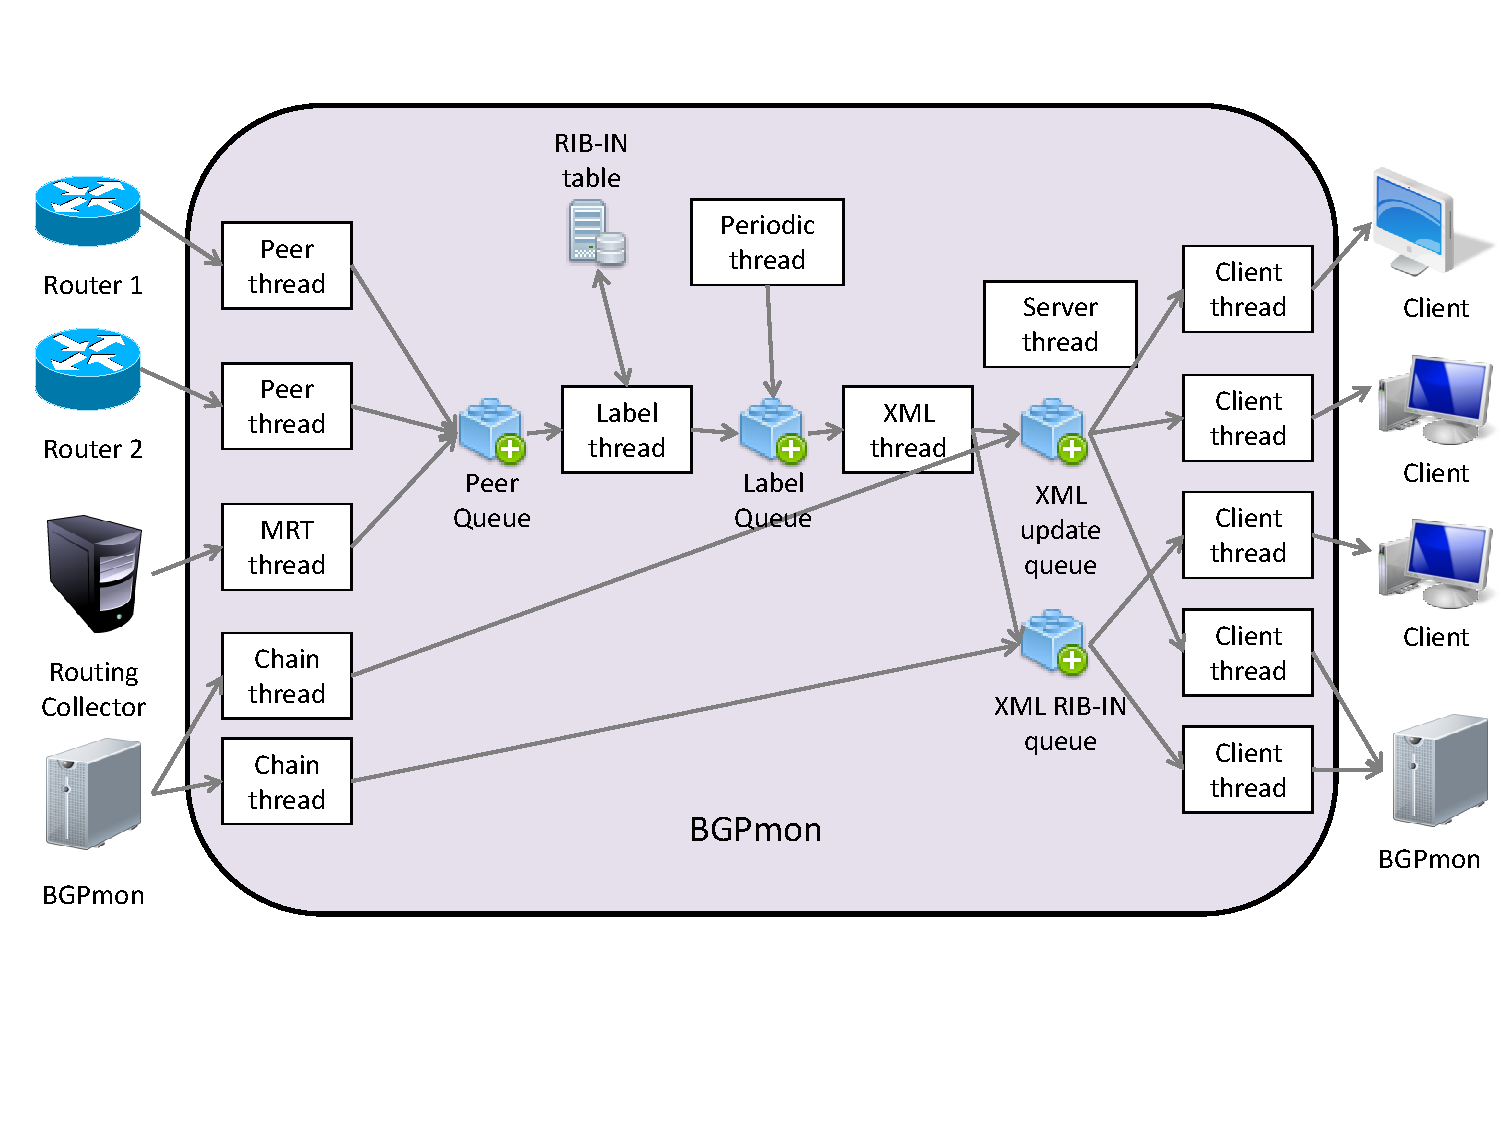
\includegraphics[scale=0.50]{figs/BGPmon-architecture.pdf}
%\caption{BGPmon architecture.}
%\label{architecturediagram}
%\end{figure*}

To support hundreds of peer routers and clients, one would like to scale out across multiple systems by adding more collectors and distributing the services. 
At the same time, a client should see a single monitoring service and be unaware that the implementation of the service may be done through multiple collectors. 
Our approach is based on publish/subscribe overlay networks that consist of brokers, publishers, and subscribers. 
The brokers form the overlay network, allowing publishers to send event streams to the overlay network and allowing subscribers to receive event streams from the overlay network. 
Publishers and subscribers interact only with brokers, not with each other, allowing the overlay network to insulate publishers and subscribers from each other. 

To improve fault tolerance, multiple brokers may monitor the same or different peers in an AS, yet appear to a client application as a single subscription. 
This allows critical applications to continue to receive event streams in the case of a failure of a peer, monitor, or broker. 
Our system implementation begins with BGPmon, a simple monitoring system now available that incorporates all three functions: publish, broker, and subscribe. 


%\section{Configuration Module}
\label{sec:config}

Configuration of BGPmon is entirely via command line interface which is very similar to a cisco router. Internally all the configurations will be stored in a XML file which can be loaded later. The configuration of a module corresponds to a  part of the XML file. In a high level, configuration module builds a bridge between main program and all the other modules in oder to facilitate the configuration management. 
More specifically, configuration module mainly consists of 3 parts.
First configuration module provides a facade to main program that allows it to read, save and backup XML configuration file without knowing the details of other modules . Secondly configuration module provides some XML utility functions to other modules as each of them needs the same set of functions to read configuration from XML file and save configuration into XML file. At last, configuration module is also a centralized place to define the XPaths of  all the configuration. 
  
  
 \subsection{Read, Save and Backup XML Configuation File} 
Configuration module provides the following 3 functions to main program:
 \begin{itemize}
 	\item{\emph{ readConfigFile: } This facade function is called by main program to load the configuration into memory from XML file. Instead of direct reading the XML configuration file it delegate reading functions to each module. In other words, each module provides a reading configuration function to load its own configuration from XML file and the facade function just needs to call these read functions in order to load all the configuration.
	If the XML configuration file is corrupted, this function will try to load as much as possible into memory and return a error code .}
	\item{\emph{ saveConfigFile:} This facade function is called by main program and login module to write the configuration from memory into XML file. Similar to \emph{ readConfigFile}, it doesn't directly write the configuration into XML file. Each module provides a writing configuration function to write its own configuration into XML file and this facade function just calls them one by one.}   
	\item{\emph{ backupConfigFile:} This function is called by main program to back up the current configuration file. It is called typically when the current configuration file is corrupted.}
	We described in details how main program uses the 3 functions in section \ref{sec:main}.
\end{itemize}  
 
  \subsection{XML Utility Functions} 
Configuration module provides a couple of get and set functions to read and write XML file.  The caller of these functions needs to pass in the XPath to locate a particular configuration item.
These get functions can return the configuration item in a specified data type and check the value against the specified conditions. For example, the caller can specify to get a configuration item in integer and check if the value is between 0 and 10. If this configuration item in XML file cannot be converted to a integer or its value is larger than 10, a error code will be returned.
 
  \subsection{XPath Definitions} 
  Each module needs to define a bunch of XPaths in order to read its own configurations from XML file.  For example, for the clients management module it configurations look like this:
     \begin{verbatim}
	<BGPmon>
    <CLIENTS>
       <LISTEN_ADDR>ipv4loopback</LISTEN_ADDR>
       <LISTEN_PORT>50001</LISTEN_PORT>
       <ENABLED>0</ENABLED>
       <MAX_CLIENTS>10000</MAX_CLIENTS>
    </CLIENTS>
	</BGPmon>
\end{verbatim}
As a result, clients management module needs to define 4 XPaths for the 4 items: LISTEN\_ADDR, LISTEN\_PORT, ENABLED and MAX\_CLIENTS. In order to get the 4 values,  clients management module needs to call the get functions mentioned before and pass in the XPaths. The XPath definitions of all modules can be found in Config\/configdefaults.h.
  
  
  \subsection{Design Philosophy} 
  As each module has the best knowledge of its own con�guration, our design divides the entire con�guration of BGPmon into a couple of small pieces according to the division of modules. Each module only handles it own piece. In this way, the changes of con�guration will be localized inside one module and none of them will be exposed to main program or other modules. XML utility functions are de�ned here as most of modules need them to handle the XML �le. Also in order to manage all the XPaths of modules e?ciently, they are centralized stored in the con�guration module. The last design issue here is about default con�guration. There are 2 reasons why we need this default con�guration.
   \begin{itemize}
 	\item{ It includes the minimal set of con�guration to start BGPmon for this �rst time. For 	example, the command line interface needs a default enable password and a default port to
	listen on even if there is no con�guration yet.}
	\item{ It provides the defaults for all the optional con�guration. For example, the BGP
	version of peer con�guration is optional and the default value will be used if it is not speci�ed by the user.}   
\end{itemize}  

The default con�guration of BGPmon can be found in site defaults.h. It can be changed by editing this �le and then recompile BGPmon. And default con�guration will be overwritten by the con�guration via command line interface.

%  As each module has the best knowledge of its own configurations, our design divides the entire configurations of BGPmon into a couple of small pieces according to the division of modules. Each module only handles it own piece.
%  In this way, the changes of configurations will be localized inside one module and none of them will be exposed to main program or other modules. 
%  XML utility functions are defined here as most of modules need them to handle the configurations in XML file. Also in order to manage all the XPaths of modules efficiently, they are  centralized stored in the configuration module.  
%    
%The BGPmon configuration parameters are divided into four classes.   First,  \emph{Peering Parameters} control all actions related to BGP peering sessions.   These parameters are discussed in Section~\ref{sec:config:peers}.     Second,  \emph{Client Parameters} control who can receive data from BGPmon.   These parameters are discussed in Section~\ref{sec:config:clients}.  Third, \emph{Chaining Parameters} instruct this BGPmon to form chains by connecting to other BGPmon instances.  These parameters are discussed in Section~\ref{sec:config:chains}.   Finally, \emph{General Parameters} control administrative access to BGPmon,  queue management, and other BGPmon system specific settings.   These parameters are discussed in Section~\ref{sec:config:general}.  

%The resulting BGPmon configuration file has the following format is shown in Figure \ref{fig:config:overview}. 

%\begin{figure}[!htb]
%\begin{verbatim}
%<BGPmon>
%     <Peering>
%          See Peering Configuration Parameter Section
%     </Peering>
%     <Clients>
%          See Client Configuration Parameter Section
%     </Clients>
%     <Chains>
%          See Chaining Configuration Parameter Section
%     </Chains>
%     <General>
%          See General Configuration Parameter Section
%     </General>
%</BGPmon>
%\end{verbatim}
%\caption{BGPmon Configuration Overview}
%\label{fig:config:overview}
%\end{figure}

%\subsection{Peering Configuration Parameters}
%\label{sec:config:peers}

%\begin{figure}[!htb]
%\begin{verbatim}
%<Peering>
%     <PEER_DEFAULTS>
%          Peer Settings
%     </PEER_DEFAULTS>
%     <PEER>
%          Peer Settings
%     </PEER>
%     ....
%     <PEER>
%            Peer Settings
%     </PEER>
%</Peering>
%\end{verbatim}
%\caption{Peering Configuration Overview}
%\label{fig:config:peer:overview}
%\end{figure}

%\emph{Peering Parameters} control all actions related to BGP peering sessions.   This is the largest and most complex configuration section.      Peering parameters are divided into three broad classes.   

%First,  there are a set of mandatory settings with compiled defaults.     The BGP version number is an example of a mandatory setting with a compiled default.    The BGP version number is a required part of some BGP messages and BGPmon must know the version number to implement the protocol correctly.     However,  most routers at the time of this writing to use version 4.   

%

%

%\begin{figure}[!htb]
%\begin{verbatim}

%<MONITOR_ADDRESS AFI=NUMBER>   
%     ADDRESS  - DEFAULT TO ADDRESS OF SOME INTERFACE 
%</MONITOR_ADDRESS>

%<MONITOR_PORT>
%    PORT_NUMBER - DEFAULT to Port 128
%</MONITOR_PORT>

%<MONITOR_VERSION>
%   BGP_VERSION_NUMBER> - DEFAULT to 4
%</MONITOR_VERSION>

%\end{verbatim}
%\caption{Mandatory - With Default}
%\label{fig:config:peer:settings}
%\end{figure}

%\begin{figure}[!htb]
%\begin{verbatim}
%<MONITOR_ADDRESS AFI=NUMBER>   
%     ADDRESS  - DEFAULT TO ADDRESS OF FIRST INTERFACE 
%</MONITOR_ADDRESS>

%<MONITOR_PORT>
%    PORT_NUMBER - DEFAULT to Port 128
%</MONITOR_PORT>

%<MONITOR_VERSION>
%   BGP_VERSION_NUMBER> - DEFAULT to 4
%</MONITOR_VERSION>
%\end{verbatim}
%\caption{Mandatory - With Default}
%\label{fig:config:peer:settings}
%\end{figure}

%\subsection{Client Configuration Parameters}
%\label{sec:config:clients}

%\emph{Client Parameters} control who can receive data from BGPmon.

%\subsection{Chaining Configuration Parameters}
%\label{sec:config:chains}

%\emph{Chaining Parameters} instruct this BGPmon to form chains by connecting to other BGPmon instances. 

%\subsection{General Parameters}
%\label{sec:config:general}

%\emph{General Parameters} control administrative access to BGPmon,  queue management, and other BGPmon system specific settings.


\section{Configuration Module}
\label{sec:config}

Configuration of BGPmon is entirely via command line interface which is very similar to a cisco router. Internally all the configurations will be stored in a XML file which can be loaded later. The configuration of a module corresponds to a  part of the XML file. In a high level, configuration module builds a bridge between main program and all the other modules in oder to facilitate the configuration management. 
More specifically, configuration module mainly consists of 3 parts.
First configuration module provides a facade to main program that allows it to read, save and backup XML configuration file without knowing the details of other modules . Secondly configuration module provides some XML utility functions to other modules as each of them needs the same set of functions to read configuration from XML file and save configuration into XML file. At last, configuration module is also a centralized place to define the XPaths of  all the configuration. 
  
  
 \subsection{Read, Save and Backup XML Configuation File} 
Configuration module provides the following 3 functions to main program:
 \begin{itemize}
 	\item{\emph{ readConfigFile: } This facade function is called by main program to load the configuration into memory from XML file. Instead of direct reading the XML configuration file it delegate reading functions to each module. In other words, each module provides a reading configuration function to load its own configuration from XML file and the facade function just needs to call these read functions in order to load all the configuration.
	If the XML configuration file is corrupted, this function will try to load as much as possible into memory and return a error code .}
	\item{\emph{ saveConfigFile:} This facade function is called by main program and login module to write the configuration from memory into XML file. Similar to \emph{ readConfigFile}, it doesn't directly write the configuration into XML file. Each module provides a writing configuration function to write its own configuration into XML file and this facade function just calls them one by one.}   
	\item{\emph{ backupConfigFile:} This function is called by main program to back up the current configuration file. It is called typically when the current configuration file is corrupted.}
	We described in details how main program uses the 3 functions in section \ref{sec:main}.
\end{itemize}  
 
  \subsection{XML Utility Functions} 
Configuration module provides a couple of get and set functions to read and write XML file.  The caller of these functions needs to pass in the XPath to locate a particular configuration item.
These get functions can return the configuration item in a specified data type and check the value against the specified conditions. For example, the caller can specify to get a configuration item in integer and check if the value is between 0 and 10. If this configuration item in XML file cannot be converted to a integer or its value is larger than 10, a error code will be returned.
 
  \subsection{XPath Definitions} 
  Each module needs to define a bunch of XPaths in order to read its own configurations from XML file.  For example, for the clients management module it configurations look like this:
     \begin{verbatim}
	<BGPmon>
    <CLIENTS>
       <LISTEN_ADDR>ipv4loopback</LISTEN_ADDR>
       <LISTEN_PORT>50001</LISTEN_PORT>
       <ENABLED>0</ENABLED>
       <MAX_CLIENTS>10000</MAX_CLIENTS>
    </CLIENTS>
	</BGPmon>
\end{verbatim}
As a result, clients management module needs to define 4 XPaths for the 4 items: LISTEN\_ADDR, LISTEN\_PORT, ENABLED and MAX\_CLIENTS. In order to get the 4 values,  clients management module needs to call the get functions mentioned before and pass in the XPaths. The XPath definitions of all modules can be found in Config\/configdefaults.h.
  
  
  \subsection{Design Philosophy} 
  As each module has the best knowledge of its own con�guration, our design divides the entire con�guration of BGPmon into a couple of small pieces according to the division of modules. Each module only handles it own piece. In this way, the changes of con�guration will be localized inside one module and none of them will be exposed to main program or other modules. XML utility functions are de�ned here as most of modules need them to handle the XML �le. Also in order to manage all the XPaths of modules e?ciently, they are centralized stored in the con�guration module. The last design issue here is about default con�guration. There are 2 reasons why we need this default con�guration.
   \begin{itemize}
 	\item{ It includes the minimal set of con�guration to start BGPmon for this �rst time. For 	example, the command line interface needs a default enable password and a default port to
	listen on even if there is no con�guration yet.}
	\item{ It provides the defaults for all the optional con�guration. For example, the BGP
	version of peer con�guration is optional and the default value will be used if it is not speci�ed by the user.}   
\end{itemize}  

The default con�guration of BGPmon can be found in site defaults.h. It can be changed by editing this �le and then recompile BGPmon. And default con�guration will be overwritten by the con�guration via command line interface.

%  As each module has the best knowledge of its own configurations, our design divides the entire configurations of BGPmon into a couple of small pieces according to the division of modules. Each module only handles it own piece.
%  In this way, the changes of configurations will be localized inside one module and none of them will be exposed to main program or other modules. 
%  XML utility functions are defined here as most of modules need them to handle the configurations in XML file. Also in order to manage all the XPaths of modules efficiently, they are  centralized stored in the configuration module.  
%    
%The BGPmon configuration parameters are divided into four classes.   First,  \emph{Peering Parameters} control all actions related to BGP peering sessions.   These parameters are discussed in Section~\ref{sec:config:peers}.     Second,  \emph{Client Parameters} control who can receive data from BGPmon.   These parameters are discussed in Section~\ref{sec:config:clients}.  Third, \emph{Chaining Parameters} instruct this BGPmon to form chains by connecting to other BGPmon instances.  These parameters are discussed in Section~\ref{sec:config:chains}.   Finally, \emph{General Parameters} control administrative access to BGPmon,  queue management, and other BGPmon system specific settings.   These parameters are discussed in Section~\ref{sec:config:general}.  

%The resulting BGPmon configuration file has the following format is shown in Figure \ref{fig:config:overview}. 

%\begin{figure}[!htb]
%\begin{verbatim}
%<BGPmon>
%     <Peering>
%          See Peering Configuration Parameter Section
%     </Peering>
%     <Clients>
%          See Client Configuration Parameter Section
%     </Clients>
%     <Chains>
%          See Chaining Configuration Parameter Section
%     </Chains>
%     <General>
%          See General Configuration Parameter Section
%     </General>
%</BGPmon>
%\end{verbatim}
%\caption{BGPmon Configuration Overview}
%\label{fig:config:overview}
%\end{figure}

%\subsection{Peering Configuration Parameters}
%\label{sec:config:peers}

%\begin{figure}[!htb]
%\begin{verbatim}
%<Peering>
%     <PEER_DEFAULTS>
%          Peer Settings
%     </PEER_DEFAULTS>
%     <PEER>
%          Peer Settings
%     </PEER>
%     ....
%     <PEER>
%            Peer Settings
%     </PEER>
%</Peering>
%\end{verbatim}
%\caption{Peering Configuration Overview}
%\label{fig:config:peer:overview}
%\end{figure}

%\emph{Peering Parameters} control all actions related to BGP peering sessions.   This is the largest and most complex configuration section.      Peering parameters are divided into three broad classes.   

%First,  there are a set of mandatory settings with compiled defaults.     The BGP version number is an example of a mandatory setting with a compiled default.    The BGP version number is a required part of some BGP messages and BGPmon must know the version number to implement the protocol correctly.     However,  most routers at the time of this writing to use version 4.   

%

%

%\begin{figure}[!htb]
%\begin{verbatim}

%<MONITOR_ADDRESS AFI=NUMBER>   
%     ADDRESS  - DEFAULT TO ADDRESS OF SOME INTERFACE 
%</MONITOR_ADDRESS>

%<MONITOR_PORT>
%    PORT_NUMBER - DEFAULT to Port 128
%</MONITOR_PORT>

%<MONITOR_VERSION>
%   BGP_VERSION_NUMBER> - DEFAULT to 4
%</MONITOR_VERSION>

%\end{verbatim}
%\caption{Mandatory - With Default}
%\label{fig:config:peer:settings}
%\end{figure}

%\begin{figure}[!htb]
%\begin{verbatim}
%<MONITOR_ADDRESS AFI=NUMBER>   
%     ADDRESS  - DEFAULT TO ADDRESS OF FIRST INTERFACE 
%</MONITOR_ADDRESS>

%<MONITOR_PORT>
%    PORT_NUMBER - DEFAULT to Port 128
%</MONITOR_PORT>

%<MONITOR_VERSION>
%   BGP_VERSION_NUMBER> - DEFAULT to 4
%</MONITOR_VERSION>
%\end{verbatim}
%\caption{Mandatory - With Default}
%\label{fig:config:peer:settings}
%\end{figure}

%\subsection{Client Configuration Parameters}
%\label{sec:config:clients}

%\emph{Client Parameters} control who can receive data from BGPmon.

%\subsection{Chaining Configuration Parameters}
%\label{sec:config:chains}

%\emph{Chaining Parameters} instruct this BGPmon to form chains by connecting to other BGPmon instances. 

%\subsection{General Parameters}
%\label{sec:config:general}

%\emph{General Parameters} control administrative access to BGPmon,  queue management, and other BGPmon system specific settings.


 \section{Peering Module}
\label{sec:peering}

Peering module manages the configuration for all peers and maintains peering sessions for enabled peers. Every peer has its own configuration that can be changed via command line interface. 
But only enabled peer will have one and only one peering session that is established by using the peer's configuration. If the peer's configuration changes after its peering session gets established, some of the new changes will not be applied to the established peering session immediately. For instance, the changes of monitor side address and port cannot be applied to the existing peering session. This kind of changes can only take effect by closing the existing session and opening a new session.

Each peering session is a separate thread that basically maintains a BGP finite state machine such as initialize a tcp connection, exchange BGP open and keepalive messages with the peer and receives BGP update messages from
the peer. It also write all messages between BGPmon and the peer into the Peer Queue. There are 3 types of messages can be added into Peer Queue: messages from peer(BMF type 2), messages to peer(BMF type 1) and FSM state changes(BMF type 6).     
 
The details of peer configuration and peering session are discussed below. 

%In addition,  the peering module maintains statistics about each peer so that other modules such as the Periodic Module can report on the peer status.
%Once the socket has been created,  each peering thread maintains a BGP finite state machine(FSM) which has five states Idle, Connect, OpenSent, OpenConfirm and Established. Compared to the complete BGP finite state machine, the state 'Active' is not implemented in our system because the peering thread always initiates the connection actively and simply drops all the incoming connection from the peering routers for the security purpose.

\subsection{Peer Configuration}
Similar to BGP configuration in cisco IOS, we use peer group to simplify the peer configuration in BGPmon. If a number of peers share a common set of configuration, peer group can simplify configuration greatly. With a peer group that has the common set of configuration, to add a new peer one only needs to assign it to the existing peer group and specify a few fields if needed. Those specified fields will overwrite the same fields from the peer group. But all the other fields from the peer group will be inherited by the peer. 

Different from cisco IOS, every peer must be associated with a peer group in BGPmon. If one doesn't specify the peer group for a peer explicitly, this peer will be assign to the default peer group that holds the default configuration. The default peer group is created when BGPmon starts. In BGPmon, every user-created peer group is also inherited from the default peer group by default and it cannot be changed. The fields specified in the user-created peer group overwrites those from default peer group.

In detail, peering module maintains 2 arrays: one array stores all peers and another stores all peer groups. Each peer in the first array holds a reference to a peer group in the second array.  The default peer group is always created at first in the peer group array as it will be referred by any user-created peer group.  Figure \ref{fig:peerandpeergroup} shows the relationship between peers and peer gourps. In the example, there are 3 peers and 3 peer groups including the default peer group. The arrows indication the relationship between them. Peer1 has it own values for configure item A and B, so those values overwrite the values in its peer group "Group2". As a net result, PA1 and PB1 will be the final values for peer1. Peer2 belongs to default peer group directly and it doesn't have its own value for item B, so peer2 inherits the value of item B from default peer group and has PA2 and DefaultB as its final values. Similar peer 3 doesn't have its own value for item A and its peer group(Group1) doesn't have the value either, so peers inherits the value of item A from default peer group. Finally peer3 has DefaultA and PB3 as it configure values.

\begin{figure}[!htb]
\centering
\scalebox{0.4}{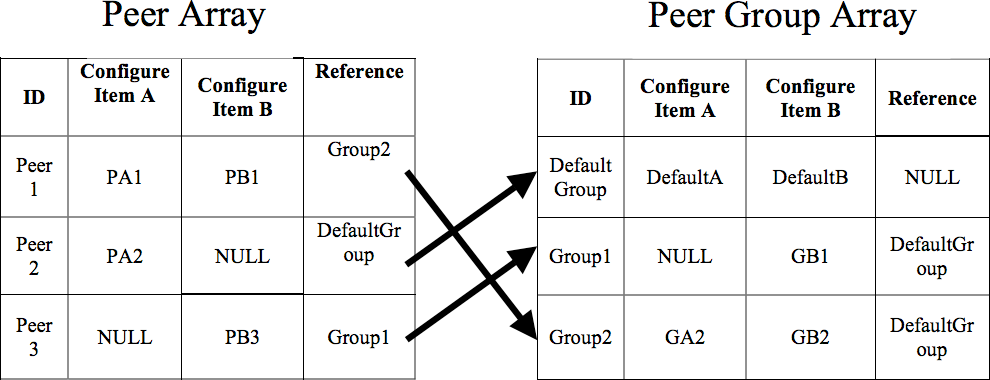
\includegraphics{figs/peerandpeergroup.pdf}}
\caption{An example of Peers and Peer Groups}
\label{fig:peerandpeergroup}
\end{figure}

From the above example, you can see the structures of peers and peer groups share the same set of configure items. In our design, peer structure and peer group structure share the same substructure "configuration" that includes all the configure items.  
Specifically peer structure consists of three parts:
\begin{itemize}
\item{\emph{Peer ID:}  It is the identifier of a peer, starting from 0. It is also the index of a peer in the array.} 

\item{\emph{Session ID:} It is  the identifier of a peering session that is associated with a peer, starting from 0. For the disabled peer, it is -1. Peering session will be discussed in the next subsection.}

\item{\emph{Configuration Substructure:} It contains all configure items needed in peer configuration.}  
\end{itemize}
And peer group structure also consists of three parts:
\begin{itemize}
\item{\emph{Peer Group ID:}  It is the identifier of a peer group, starting from 0. It is also the index of a peer group in the array.} 

\item{\emph{Peer Group Name:} It is the name of a peer group.}

\item{\emph{Configuration Substructure:} It is same as the configuration substructure in peer structure.}  
\end{itemize}
Configuration substructure includes all the configure items which are needed by peering session establishment, labeling module and periodic event handling module. Figure \ref{fig:configurationSub} shows the details of configuration substructure. All of these configure items except "routerRefreshAction" and "labelAction" are used to establish a peering session. "routerRefreshAction" is used by periodic event handling module and "labelAction" is used by labeling module.
\begin{figure*}
\centering
\scalebox{1}{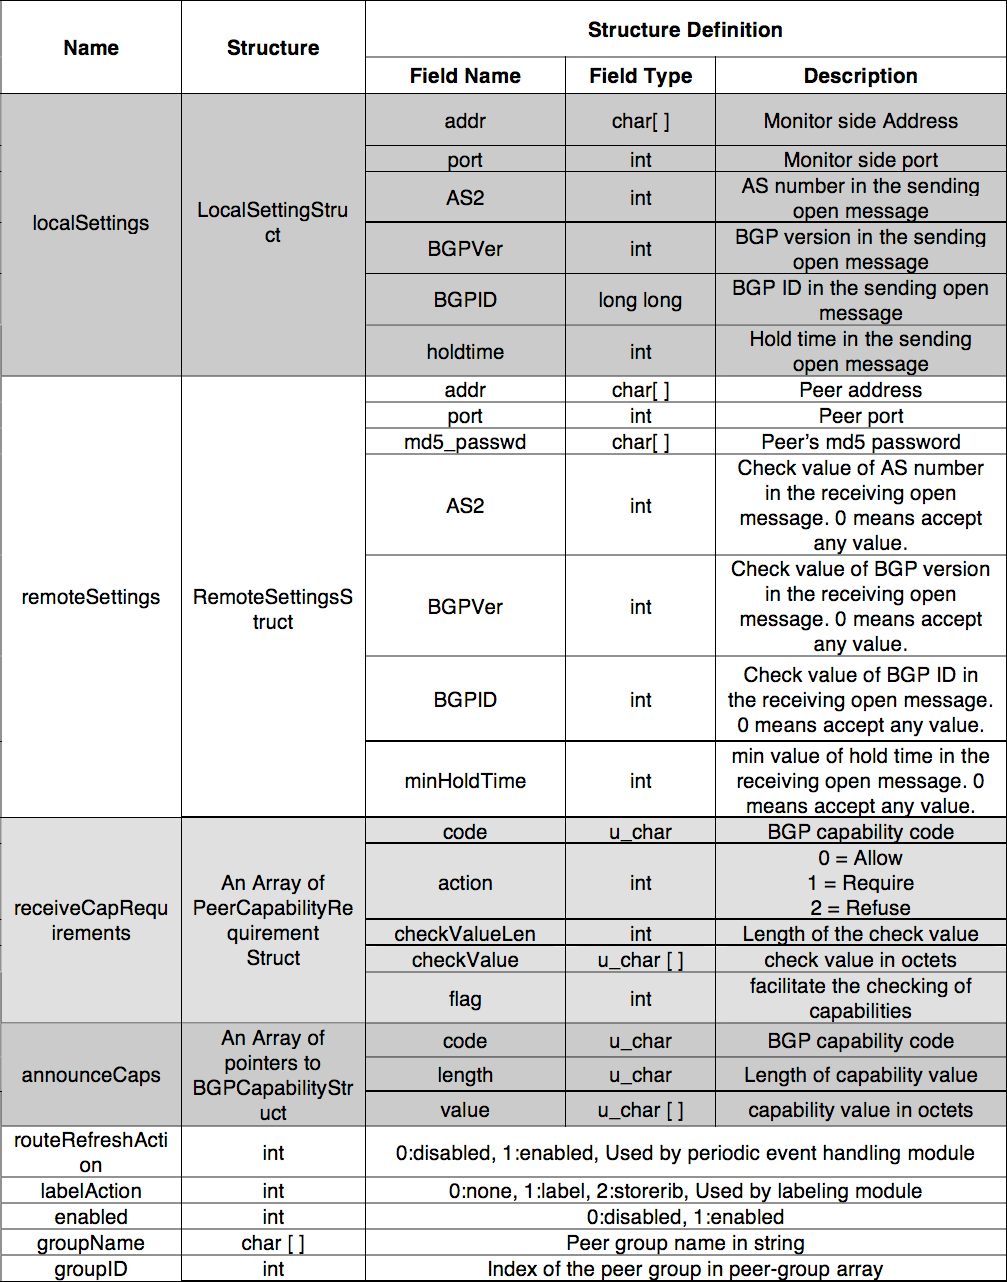
\includegraphics{figs/configurationSub.pdf}}
\caption{Configuration Substructure}
\label{fig:configurationSub}
\end{figure*}

Peering module also provides a bunch of functions to create, delete, read and write peers and peer groups.  Command line interface uses these functions to manipulate peer configuration. We have discussed the peer configuration so far. Next peering session will be discussed. 

\subsection{Peering  Session}
Peering module maintains an array that holds the data for all peering sessions and each element in this array is a "Session" structure. "Session" structure is not only used by peering module but also used by labeling module, periodic event handling module and XML module.
As we mentioned each enabled peer has its own thread and these threads create "Session" structures in the array and uses them to establish and maintain the peering sessions. In each peer's thread, a peering session gets established by using the latest configuration of that peer. When a peering session is established, all the configure items that are used to establish the session will be saved in the "Session" structure. After that, any changes in those configure items via command line interface will not take effect until the peering session resets. And the peering session could be reset in the following 2 cases.
\begin{itemize}
\item{Users reset the peering session explicitly by issuing a reset command via command line interface. This happens typically when users change some peer configuration via command line interface and want these changes to be applied immediately. } 
\item{Peering session resets by itself. For example, the underlying tcp connection failure could cause a peer session reset.  Or the peering session could be reset if the peer fails for some reason.   }  
\end{itemize}
No matter why the peering session is reset, the latest peer configuration will be used when it gets established again. 
An important design decision here is that a new "Session" structure with new session ID will be created and used by the thread every time a peering session is reset.  Note even the thread is using the new "Session" structure, the old one will still stay in the session array for a while until it is not needed. We will discuss the design philosophy behind this in the next subsection.
In the remaining part of this subsection, the detail of "Session" structure will be discussed at first and then an introduction of how to establish and maintain a peering session by using "Session" structure will be given.

\subsubsection{"Session" Structure}
\label{sec:peering:sessionstructure}
Most fields of a "Session" structure are related to the peering module and a few fields are related to other modules. The details are shown as follows:
\begin{itemize}

\item{\emph{sessionID:} is the identification of a peering session which starts from 0. It is also the index of a peering session in the array.}

\item{\emph{ConfigInUse substructure:} is same as the configuration substructure shown in Figure \ref{fig:configurationSub}.   It is basically a copy of peer configuration when peering session gets established. It will not be changed once the peering session gets established. This substructure is important if one wants to know what are the differences between the latest peer configuration and the configuration used to establish the peering session.}

\item{\emph{FSM substructure:} is a group of fields that are used to maintain the BGP Finite State Machine (FSM) such as state of FSM, socket and a couple of timers. Figure \ref{fig:FSMSub} shows the details of FSM substructure.}
\begin{figure*}
\centering
\scalebox{0.9}{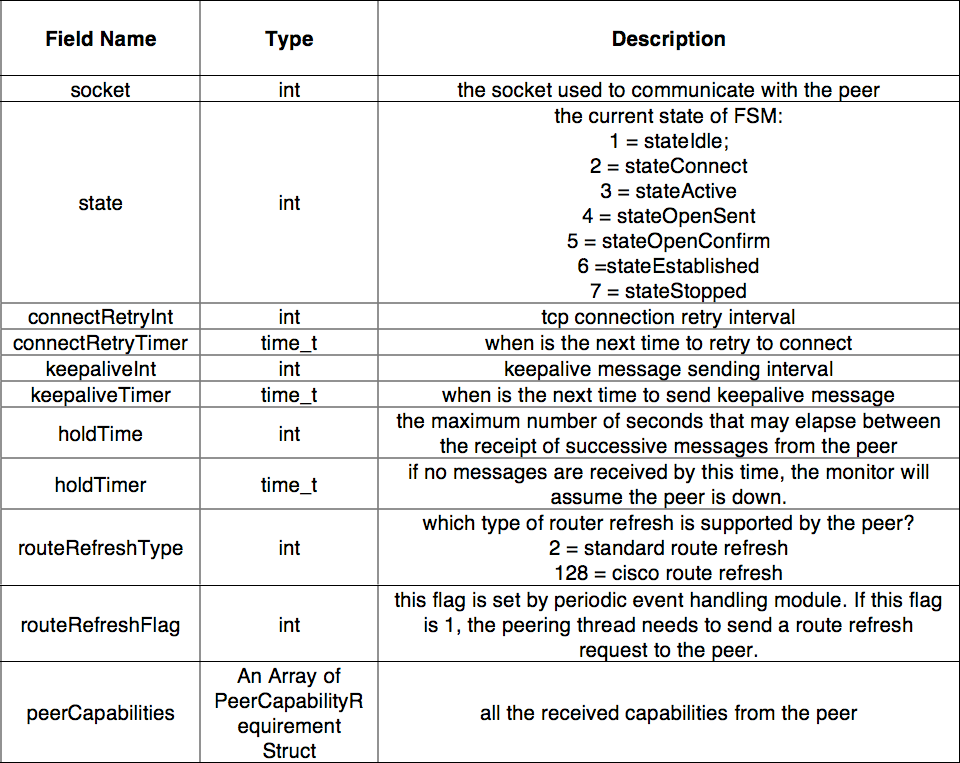
\includegraphics{figs/FSMSub.pdf}}
\caption{FSM Substructure}
\label{fig:FSMSub}
\end{figure*}

\item{\emph{Statistics substructure:} is a group of fields related to the peer's statistics such as the time of last session reset and the number of received updates. Figure \ref{fig:StatSub} shows the details of statistics substructure}
\begin{figure*}
\centering
\scalebox{0.9}{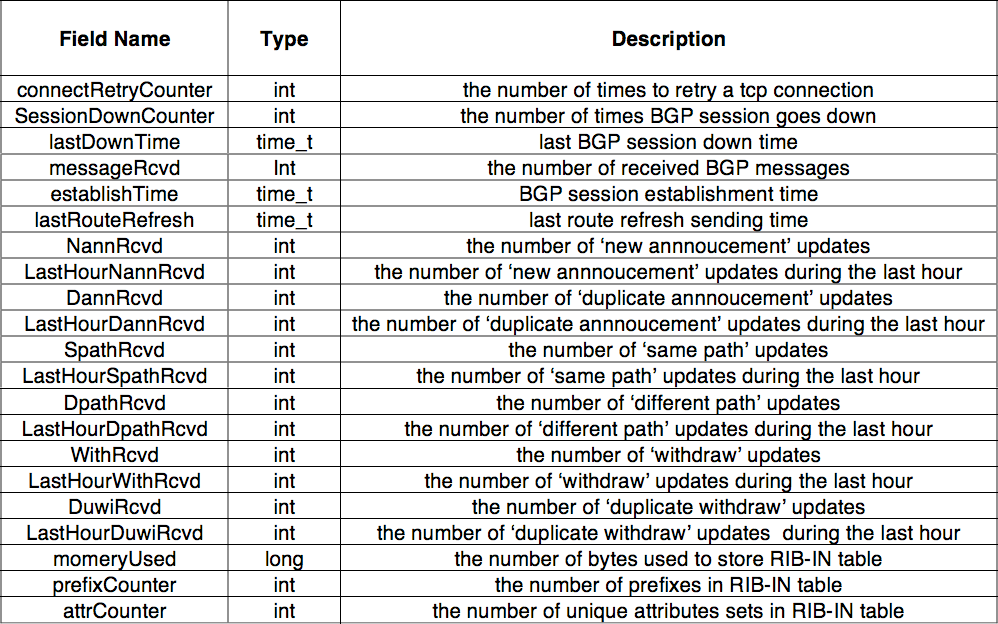
\includegraphics{figs/StatSub.pdf}}
\caption{Statistics Substructure}
\label{fig:StatSub}
\end{figure*}

\item{\emph{peerQueueWriter:} is used to write the messages exchanged between BGPmon and the peer into the queue. }

\item{\emph{sessionStringOutgoing:} is a XML string generated by peering module. It is used by XML module as the common XML header of all outgoing messages. It consists of 2 triples: Source triple and Destination triple.
Source triple contains monitor side address port and AS number.  Destination triple contains peer's address, port and AS number.   }

\item{\emph{sessionStringIncoming:} is similar to sessionStringOutgoing. It is a common XML header for all incoming messages. In this XML string, source triple contains peer address port and AS number.  Destination triple contains monitor side address, port and AS number. }

\item{\emph{PrefixTable Substructure and AttrTable Substructure:} are used to maintain a RIB table. They are initialized by peering module and populated by labeling module. The detail of them will be discussed in Section \ref{sec:labeling}. }

\item{\emph{reconnectFlag:} is used to reset a peering session and set by command line interface. This flag is typically set when a user wants the changes of peer configuration to be applied. }

\item{\emph{lastAction:} is a timestamp that indicates when the last action of a peering session is. It is used to check if a peering session is running correctly. }

\end{itemize}

\subsubsection{Establish and Maintain Peering Sessions}

To establish a BGP peering session, the first step in peer's thread is to create a socket and bind it to the monitor side address and a port specified in "localSettings" of the peer configuration( See Figure \ref{fig:configurationSub}). 
Secondly, the thread needs to initiate a tcp connection to the peer actively. Similarly, the peer's address and port are specified in "remoteSettings" of the peer configuration. Note in our design the thread always initiates the connection actively and simply drops all the incoming connection from the peer for the security purpose.

Once the tcp connection is established, the thread will exchange the BGP open message with the peer. As shown in  Figure \ref{fig:configurationSub}, all the parameters(BGP version, BGP ID, AS number and holdtime) needed to create a BGP open message can be found in "localSettings" of configuration substructure. Also all announcing capabilities included in the open message can be found in "announceCaps" of configuration substructure.
Then the thread sends the created open message via the established tcp connection and waits for the incoming open message from the peer. 

Upon receiving the open message, the thread will do the following two checks.
\begin{itemize}
\item{ Check the version, AS number, Identifier and holdtime in the received open message against the expected values specified in "remoteSetting" of configuration substructure( See Figure \ref{fig:configurationSub}). }
\item{ Check the capabilities in the received open message against the capability requirements specified in "receiveCapRequirements" of the configuration substructure(Figure \ref{fig:configurationSub}). For each capability $A$ in capability requirements, there are three possible actions:  }
\begin{itemize}
\item{ \emph{Allow:} nothing needs to be done.}
\item{ \emph{Require:} check if the received capabilities contain $A$ and the value of the received capability is same as the check value is configured. If no, check fails.}
\item{ \emph{Refuse:} check if the received capabilities contain $A$ and the value of the received capability is same as the check value is configured. If yes, check fails. }
\end{itemize}
\end{itemize}
If any of these checks fails, the thread will send a notification message to the peer and close the connection.
If all the checks pass, the thread will send a keepalive message to the peer and wait for another keepalive message from the peer. Once this keepalive message is received, the BGP peering session is successfully established. 

After the peering session gets established, the thread will periodically sent out keepalive messages if holdtime is not zero and route refresh requests if configured.

Each thread also writes two types of messages into the peer queue:
\begin{itemize}
\item{BGP Message: The BGP messages exchanged with the peer are written into the peer queue. Note no 'Update' messages will be sent from BGPmon. }
\item{FSM Message: The state changes of BGP finite state machine are written into the peer queue such as from 'Idle' to 'Connect', from 'OpenConfirm' to 'Established' and so on.}
\end{itemize}
These types of messages are converted into BGPmon internal format before being written into peer queue. After conversion, the session ID in the message indicates it belongs to which peering session.

In our design, periodic event handling module centralized manages and schedules the route refresh for all the peers. Instead of sending route refresh requests by itself, periodic event handling module notifies the peering module to send route refresh requests when needed. And the field 'routeRefreshFlag' in FMS substructure(Figure \ref{fig:FSMSub}) is used to notify peering module. 

\subsection{Design Philosophy}
In the design of peering module, one important issue is how to handle changes in a peer's configuration when the peer already has a existing peering session. Most of configuration changes will only take effect by resetting the existing peering session such as changes in monitor address, port or AS number. But it is not practical to reset a peering session every time such a change happens. Probably one might want to reset the peering session after a series of changes is done. So we decided to let the user make the decision about when to reset the peering session. User can reset the peering session by issuing a command via command line interface. 

As a result of letting user make the decision when to make configuration changes take effect, it is necessary to provide the user with the difference between the latest peer configuration and the configuration used to establish the existing peering session.
This explains why we need a "ConfigInUse" substructure in a "Session" structure. The "ConfigInUse" substructure is copied from peer configuration when peering session is established and will not be changed after that.
By comparing the "ConfigInUse" of a peering session and the latest peer configuration, the user will know all the changes of a peer configuration since its peering session was established. 

Another important design issue is that a new "Session" structure with new session ID will be created and used by the thread every time a peering session is reset. The reason is related to the BGPmon architecture and the format of BMF message.
As we discussed, modules of BGPmon are connected by queues and every message in peer queue and label queue has a session ID field. 
The session ID will be used as the key to retrieve the information needed to process the BMF messages by other modules such as labeling module and XML module.
For example, XML module needs the session ID to get the XML common header("sessionStringOutgoing" and "sessionStringOutgoing" in a "Session" Structure) in order to convert a BMF message to a XML string.
In BGPmon it is possible that some BMF messages associated with old peering session are buffered in the queue after a peering session gets reset . 
In this case if the peer's thread doesn't create a new "Session" structure and simply uses the same "Session" structure, XML module will wrongly convert the BMF messages associated with old peering session by using the XML common header of new peering session.
In order to avoid this,  the peer's thread needs to create a new "Session" structure and keep the old "Session" structure when a peering session is reset. After peering session reset, the peer's thread will use the new "Session" structure and tag the new BMF messages with new session ID.
The old "Session" structure will finally be deleted after all the BMF message associated with the old peering session are processed. 
%\subsection{Data Structure}
%The single key data structure of peering module is called session. Each peering thread is attached with a session structure. The session structure consists of five parts:
%\begin{itemize}

%\item{\emph{sessionID:} is 16 bit session identification. It is started from 1 and each peering thread is associated with a unique SessionID.}

%\item{\emph{Configuration substructure:} includes all the configurations of a peer which are needed to establish the BGP session such as peer's address and AS number. It is created by configuration module. The Configuration Module will write this section and the Peering Module will only read it.}

%\item{\emph{FSM substructure:} is a set of fields which are related the BGP Finite State Machine (FSM) used to maintain the BGP session.   The Peer Module will write and read this section.   Other modules may read this section to learn the status of a peer.}

%\item{\emph{Statistics substructure:} is a group of fields related to the peer's statistics such as the time of last session reset and the number of received updates.    The Peer Module will write and read this section.   Other modules may read this section to learn statistics about this peer.}

%\item{\emph{peerQueueWriter:} It is used to write the messages received from peers to the peer queue. }

%Figure \ref{fig:sessionStruct} shows the session structure.
%%\begin{figure*}
%%\centering
%%\caption{BGPmon Internal Message Types}
%%\label{tab:sessionStruct}
%%\end{figure*}

%%\begin{figure}[!htb]
%\begin{figure}[!htb]
%\scalebox{0.56}{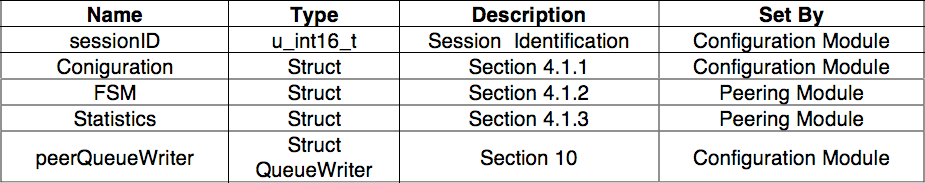
\includegraphics{figs/sessionStruct.pdf}}
%\caption{Session Structure}
%\label{fig:sessionStruct}
%\end{figure}

%%\begin{figure*}
%%\centering
%%\begin{tabular}{| l | l | l |}
%%\hline
%%sessionID & $u_int16_t $ & Session  Identification & Configuration Module\\
%%\hline
%%configuration & struct & Section 4.1.1 & Configuration Module\\
%%\hline
%%FSM & struct & Section 4.1.2 & Peering Module\\
%%\hline
%%statistics & struct & Section 4.1.3 & Peering Module\\
%%\hline
%%\end{tabular}
%%\caption{Session Structure}
%%\label{tab:sessionStruc}
%%\end{figure*}
%\end{itemize}

%\subsubsection{Configuration  SubStructure}
%Configuration SubStructure consists of six parts. 
%\begin{itemize}
%\item{\emph{BGP Open Message:}  It is the BGP open message sent to the peer in order to establish the BGP session.} 

%\item{\emph{Monitor Settings:} It contains a protocol independent address structure which is used to open the socket and a hold time used to negotiate the final hold time with the peer. }

%\item{\emph{Router Settings:} First it contains a protocol independent address structure and optional MD5 password which are used to connect to the peer. Secondly it contains the expected AS number, BGP version, BGP Identifier and minimal hold time. The received open message from the peer is checked against these expected values. }

%\item{\emph{Capability Requirements:} It contains a array of capability requirements based on the configuration. The received capabilities from the peer are checked against these capability requirements. }

%\item{\emph{Desired Configuration:} It is used to signal the peering module the changes in configuration. It will be incremented by one every time the configuration is changed by configuration module. }

%\item{\emph{Enabled:} It is used to signal the current configured peer status(pause, normal or close). It is set by configuration module.   }

%\end{itemize}
%Figure \ref{fig:configurationSub} shows the details of configuration substructure. 
%\begin{figure*}
%\centering
%\scalebox{1}{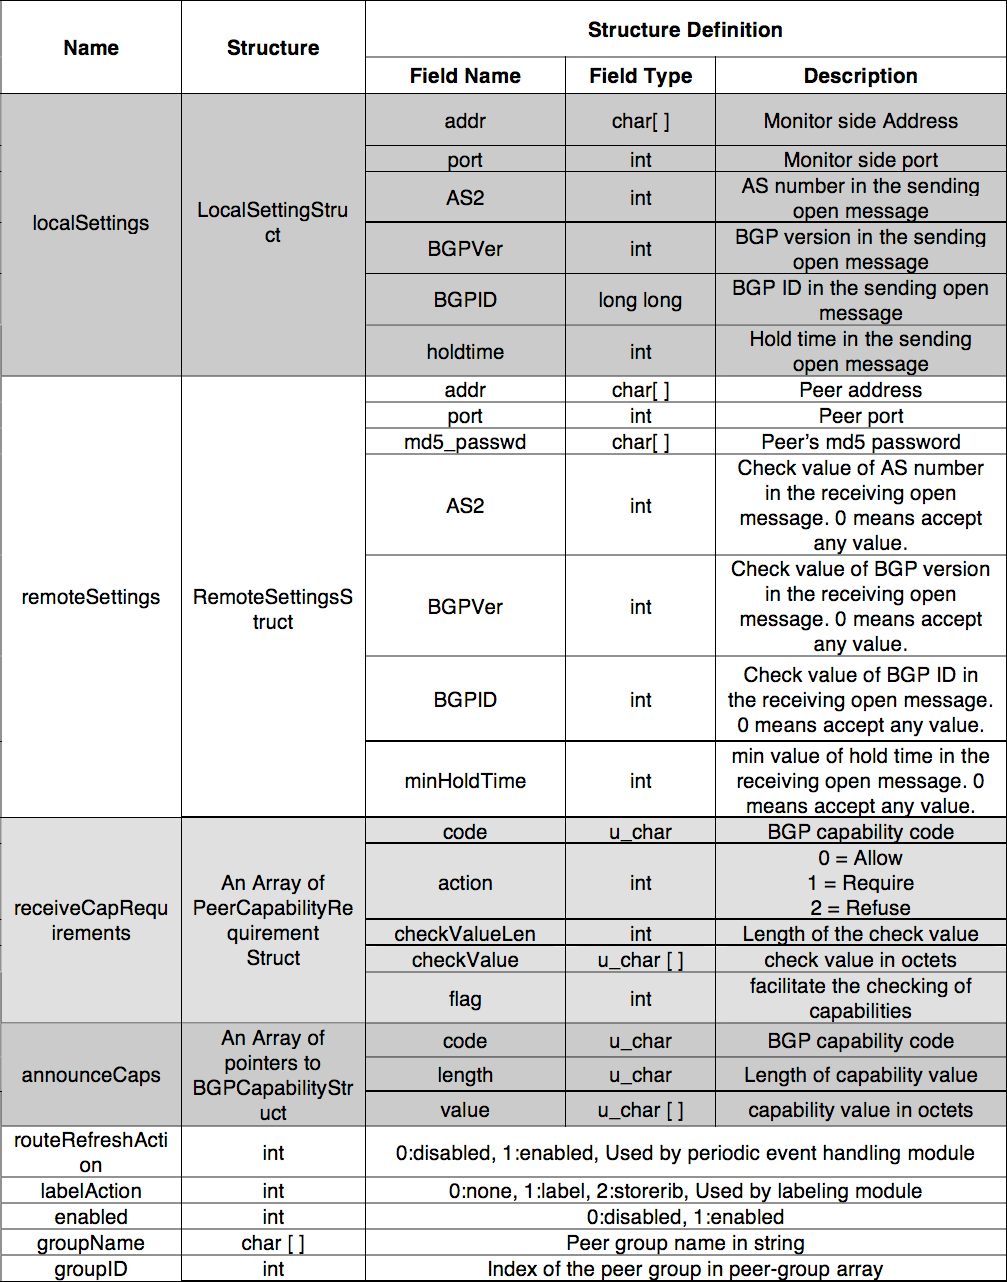
\includegraphics{figs/configurationSub.pdf}}
%\caption{Configuration Substructure}
%\label{fig:configurationSub}
%\end{figure*}

%\subsubsection{FSM SubStructure}
%FSM substructure contains all the information needed to maintain a BGP session.  It consists of a socket, the current state of FSM, and several timers.
%Figure \ref{fig:FSMSub} shows the details of FSM substructure.
%\begin{figure*}
%\centering
%\scalebox{1}{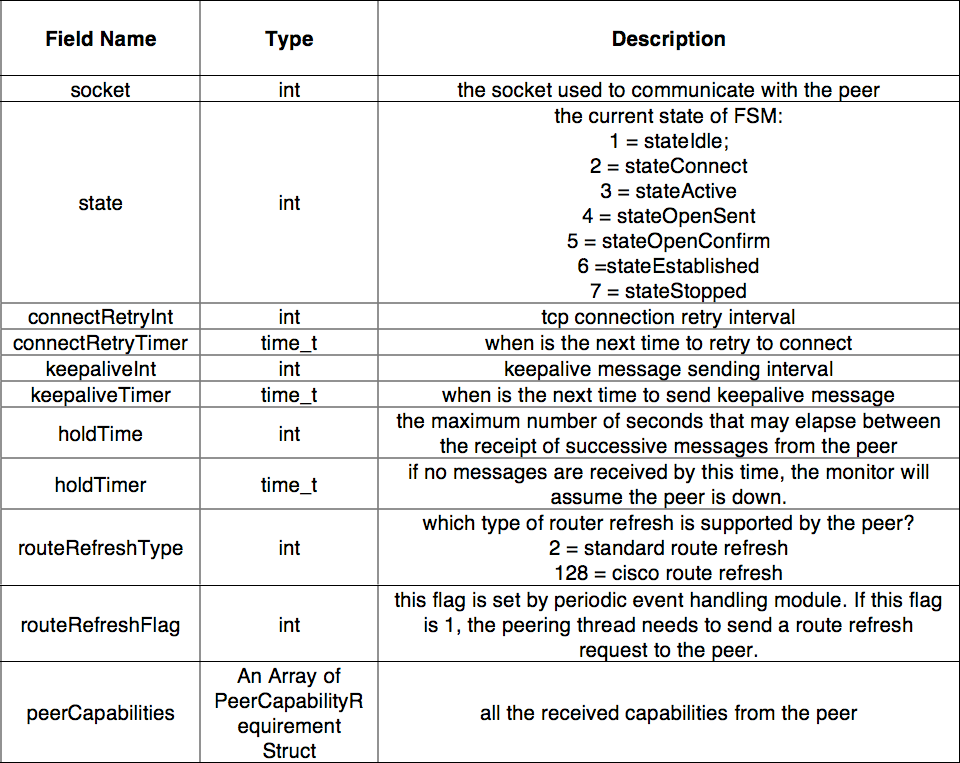
\includegraphics{figs/FSMSub.pdf}}
%\caption{FSM Substructure}
%\label{fig:FSMSub}
%\end{figure*}

%\subsubsection{Statistics SubStructure}
%Statistics substructure contains the peer's statistical information. 
%Figure \ref{fig:StatSub} shows the details of statistics substructure.
%\begin{figure*}
%\centering
%\scalebox{1}{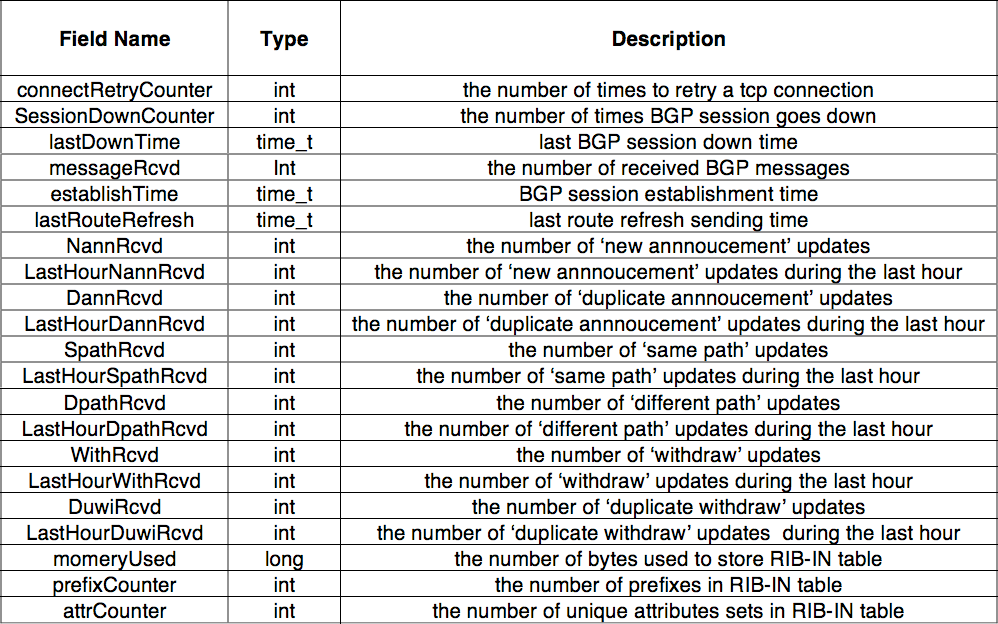
\includegraphics{figs/StatSub.pdf}}
%\caption{Statistics Substructure}
%\label{fig:StatSub}
%\end{figure*}

%\subsection{Opening and Maintaining Peering Sessions}

%% opening the socket....     note config has set address.    do not care if this is IPv4 or Ipv6 or other.
%The first step of peering thread is to create a socket and bind it to a interface and a port if configured. According to Figure \ref{fig:configurationSub}, configuration module has created monitor's protocol independent address structure.  This structure contains all the information needed to create sockets and bind sockets such as address family, socket type, address and port. So the peering thread can simply create and bind a socket with this protocol independent address structure without knowing its content such as its address family(IPv4 or IPv6) and the port number. 

%Secondly, the peering thread needs to establish the tcp connection with the router actively. Similarly, configuration module has created router's protocol independent address structure. The peering thread can establish the tcp connection by using the created socket and the router's protocol independent address structure.
%Note in our design the peering thread always initiates the connection actively and simply drops all the incoming connection from the router for the security purpose.

%Once the tcp connection is established, the peering thread will exchange the BGP open message with the peer. As we mentioned before, configuration module has created the open message and included all desired capabilities(Figure \ref{fig:configurationSub}). The peering thread just sends the created open message via the established tcp connection and waits for the incoming open message from the peer. Upon receiving the open message, the peering thread will do the following two checks.
%\begin{itemize}
%\item{ Check the version, AS number, Identifier and holdtime in the received open message against the expected values of them in the configuration substructure(Figure \ref{fig:configurationSub}). }
%\item{ Check the capabilities in the received open message against the capability requirements in the configuration substructure(Figure \ref{fig:configurationSub}). For each capability $A$ in capability requirements, there are three possible actions:  }
%\begin{itemize}
%\item{ \emph{Allow:} nothing needs to be checked.}
%\item{ \emph{Require:} check if the received capabilities contain $A$ and the value of the received capability is same as the check value is configured. If no, check fails.}
%\item{ \emph{Refuse:} check if the received capabilities contain $A$ and the value of the received capability is same as the check value is configured. If yes, check fails. }
%\end{itemize}
%\end{itemize}
%If any of these checks fails, the peering thread will send a notification message to the peer and close the connection.
%If all the checks pass, the peering thread will send a keepalive message to the peer and wait for another keepalive message from the peer. Once this keepalive message is received, the BGP session is successfully established. 

%After the BGP session gets established, the peering thread will periodically sent out keepalive messages if holdtime is not zero and route refresh requests if the peer supports it.
%   

%% sending the open message....   note config has set open message and included all desired capabilities.
%% checking the capabilities....     how does it do this?   what notifies are sent?
%%Figure \ref{fig:capstruct} show the capabilities structure used by the peering module.
%%maintaining the connection....    sending and receiving keepalives.     what if hold time is zero?   what notifies might be sent?

%Each peering thread also writes two types of messages into the peer queue:
%\begin{itemize}
%\item{BGP Message: The BGP messages sent or received by the peering threads are written into the peer queue. Note no 'Update' messages are sent from the peering thread to peering router. }
%\item{FSM Message: The state changes of BGP finite state machine made by the peering thread are written into the peer queue such as from 'Idle' to 'Connect', from 'OpenConfirm' to 'Established' and so on.}
%%\item{Peer Status Message: The states of the peer are written into the queue. The states of peer can be very simple such as the peer's address and AS number.  It also can be complex such as the BGP capabilities received from the peer. }
%\end{itemize}
%These types of messages are converted into BGPmon internal format by peering threads before being written into peer queue.

%%\subsection{Maintaining Statistics}
%% what do we maintain?     last action time,  bytes recvd, bytes sent, ??

%\subsection{Route Refresh}
%% how do we request this?
%Periodic event handling module centralized manages and schedules the route refresh for all the peers. Instead of sending route refresh requests by itself, periodic event handling module notifies the peering threads to send route refresh requests when needed. And a field 'routeRefreshFlag' in FMS substructure(Figure \ref{fig:FSMSub}) is set to notify peering thread by periodic event handling module.  Each peering thread reads this flag field after every step in FSM and it needs to send the router refresh request to the peer if this flag is set to 1. 

%% what do we do if we receive one?

%%\subsection{Closing Peering Sessions}
%%Configuration module may need to close a peering session in some cases. Similar to the route refresh case, configuration module notifies the peering thread to close a peering session by setting a field 'close flag' in FMS substructure(Figure \ref{fig:FSMSub}). Each peering thread checks this flag field after every step in FSM. If it is set to 1, the peering thread needs to send a notification message to the peer before closing the tcp connection.

%\subsection{Dynamic Configuration Change}
%The last design issue in this section is how peering thread detects the dynamic configuration changes. In our approach there are two sequence numbers associated with the configuration substructure and FSM substructure. The one in FSM substructure is called 'configurationInUse' which indicates the configuration using by peering thread. Another in configuration substructure is called 'desiredConfiguration' which indicates the latest configuration set by configuration module. 'desiredConfiguration' will be increased by configuration module when the configuration changes. Besides this two sequence numbers, there is another flag in configuration substructure called 'enable'. This flag which is et by configuration module indicates which action should be done by peering thread after a configuration change. 

%Right after every step in FSM, the peering thread will do the following checks:
%\begin{itemize}
%\item{ If 'configurationInUse' is smaller than 'desiredConfiguration', sends notification message,  clean the corresponding RIB-IN table and close the TCP connection if BGP session is established.}
%	\begin{itemize}
%	\item{If 'enable' is set to 0, pause the FSM and don't try to open a new session.}
%	\item{If 'enable' is set to 1, open a new BGP session.}
%	\item{If 'enable' is set to 2, close the thread and set the state of FSM to 7(stateStopped).}
%	\end{itemize}
%\item{ Otherwise, do nothing.}
%\end{itemize}

%%if $configurationInUse $ is smaller than $configurationInUse $. If yes, peering thread needs to restart the BGP session and also set $PeeringConf$  as same as $CurrentConf$.

%
%Obviously there is a delay between configuration module changes the configuration and peering thread uses the changed configuration. The delay depends on how long a step of FSM takes. In a extreme case, if a peering doesn't support keepalive messages, the changed configuration will not take effect until the next incoming BGP update. Such a long delay is not acceptable. In order to solve this problem, we can introduce a dedicated timer to check the configuration periodically. 

%Basically all the parts except configuration substructure in session structure are created by configuration module and then maintained by peering module. But for the configuration substructure,  it still needs to be maintained by configuration module after creation in order to support dynamically configuration. 
%More specifically, there are two steps to support dynamically configuration.
%\begin{itemize}
%\item{Configuration module changes the configuration substructure inside a session structure after the user changes the peer's configuration.}
%\item{Peering module needs to detect the changes quickly and do the corresponding actions. For example, if the peer's address changes the session must be reestablished. }
%\end{itemize}
\section{MRT module}
\label{sec:mrt}

This section describes MRT module.

\subsection{MRT overview}
Multi-threaded Routing Toolkit (MRT) format was developed to encapsulate, export, and archive routing information in a standardized data representation.  The BGP routing protocol, in particular, has been the subject of extensive study and analysis which has been significantly aided by the availability of the MRT format. 

BGPmon MRT module gives an opportunity to receive data (updates and RIBs) from Routing Collectors (RC) such as University of Oregon Route Views Project\cite{routeviews}, RIPE NCC RIS Project\cite{riperis} and others.

MRT control module consists of a single MRT server thread and multiple MRT client threads.
\begin{itemize}
\item{\emph{MRT Server Thread:} It is a TCP server that listens on a specific port and spawns one thread for each client. }
\item{\emph{MRT Client Thread:} Each client thread receives data from a TCP connection.}
\end{itemize}

\subsection{MRT Server Thread}
The main data structure of MRT control module consists of the following fields:
\begin{itemize}
\item{\emph{listenAddr:} The listening socket of server thread binds to this address.  It is a string which could be a IPv4/IPv6 address or one of four keywords (ipv4loopback, ipv4any, ipv6loopback and ipv6any). After it is intialized from configuration, it could be set via command line interface (CLI) at runtime.}
\item{\emph{listenPort:} It is the port on which server thread listens.  It is an integer.  It also could be set via command line interface(CLI) at runtime after initialization.}
\item{\emph{enabled:} It indicates the status of server thread.  If it is false, server thread stops listening but the existing clients still run. Otherwise server thread listens on 'listenPort' and accepts allowed clients. It could be set via CLI after initialization.}
\item{\emph{maxMRTclients:} It is the max number of MRT clients. It could be set via CLI after initialization. }
\item{\emph{labeAction:} Its is the label action of MRT clients}
\item{\emph{activeMRTclients:} It is the number of connected MRT clients. }
\item{\emph{nextMRTclientID:} It is the ID for the next client to connect. }
\item{\emph{rebindFlag:} If listenAddr or listenPort changes, this flag will be set to TRUE. That means the listening socket of server thread will bind to the new address or port. It is set by CLI.  }
\item{\emph{shutdown:} It is a flag to indicate whether to stop the server thread. }
\item{\emph{lastAction:} It is a timestamp to indicate the last time the thread was active. }
\item{\emph{MRTListenerThread:} Reference to MRT thread. }
\item{\emph{firstNode:} First node in list of active MRT clients} 
\item{\emph{MRTLock:} It is a pthread mutex lock used to lock the MRT info linked list when MRT clients are added or deleted. }
\end{itemize}
This structure is mainly maintained by server thread. 

\subsection{MRT Client Thread}
MRT Client Thread has:
\begin{itemize}
\item{\emph{id:} Identification number of MRT client. }
\item{\emph{addr:} MRT Client's IP address. }
\item{\emph{port:}  MRT Clients's Port number. }
\item{\emph{socket:} MRT Client's socket for reading data }
\item{\emph{connectedTime:} MRT Client's connected time in seconds. } 
\item{\emph{lastAction:} MRT Client's last action timestamp.}
\item{\emph{qWriter:} This is a queue writer (see section \ref{sec:queue}). It is used to write messages to Peering queue. }
\item{\emph{deleteMRTClient:} Flag to indicate to close the MRT Client thread}
\item{\emph{labelAction:} Default label action. }
\item{\emph{next:}  Pointer to next MRT Client node. }
\item{\emph{MRTThreadID:}  Thread reference. }
\end{itemize}

\subsection{MRT Module Peering Design}

\subsubsection{Existing/3rd Party Routing Collectors}
Although BGPmon is able to peer directly with routers, there might be existing Routing Collectors in the Internet. BGPmon is able to work with these external RCs with a few modifications to the RC software. In order to provide correct routing data to the end user, RC should send both a RIB-IN tables and updates. Before describing changes to existing Routing Collectors, we should discuss software design of Routing Collector. Despite the fact that Routing Collector peers with other routers via TCP connection, it could provide routing data to BGPmon. In our design, we assume that Routing Collector can establish multiple TCP connections to BGPmon. Moreover, we need to answer the following questions: How Routing Collector should supply routing data to BGPmon and What is the right way to do that?
\begin{itemize}
	\item{\emph{For every peering router, Routing Collector establish a TCP session and forward routing data to BGPmon:} For example shown in Figure \ref{fig:routingcollector}, if Router 2 establishes BGP peering session with Routing Collector, RC creates a single TCP connection to BGPmon. For other routers, RC should create separate connections to BGPmon. This design makes peering session management easy: if BGP session between Router 2 and Routing Collector is failed, RC should close connection to BGPmon. }
	\item{\emph{Routing Collector establish only 2 TCP connections: one is update messages stream and second - RIB-IN messages stream:} Figure \ref{fig:routingcollector} shows example of the architecture. In our design, it does not matter how many peers RC has, RC will need only 2 TCP connections to BGPmon to send routing data from Routers 1-4. }
\end{itemize}



First answer looks reasonable because of peers up/down session management: for example, if Routing Collector's BGP peering failed with Router 2 and RC closes tcp connection to BGPmon, BGPmon must erase all BGP attributes and prefixes from its routing table associated with Router 2. But in our design we choose to use second approach. The main reason of this decision - number of connections (just two) required to send update and RIB-IN messages. Another important trade-off factor - insignificant code changes/additions to Routing Collector's software. These changes adds new functions to send routing data from Routing Collector to BGPmon. 


\begin{figure*}
\centering
\scalebox{0.55}{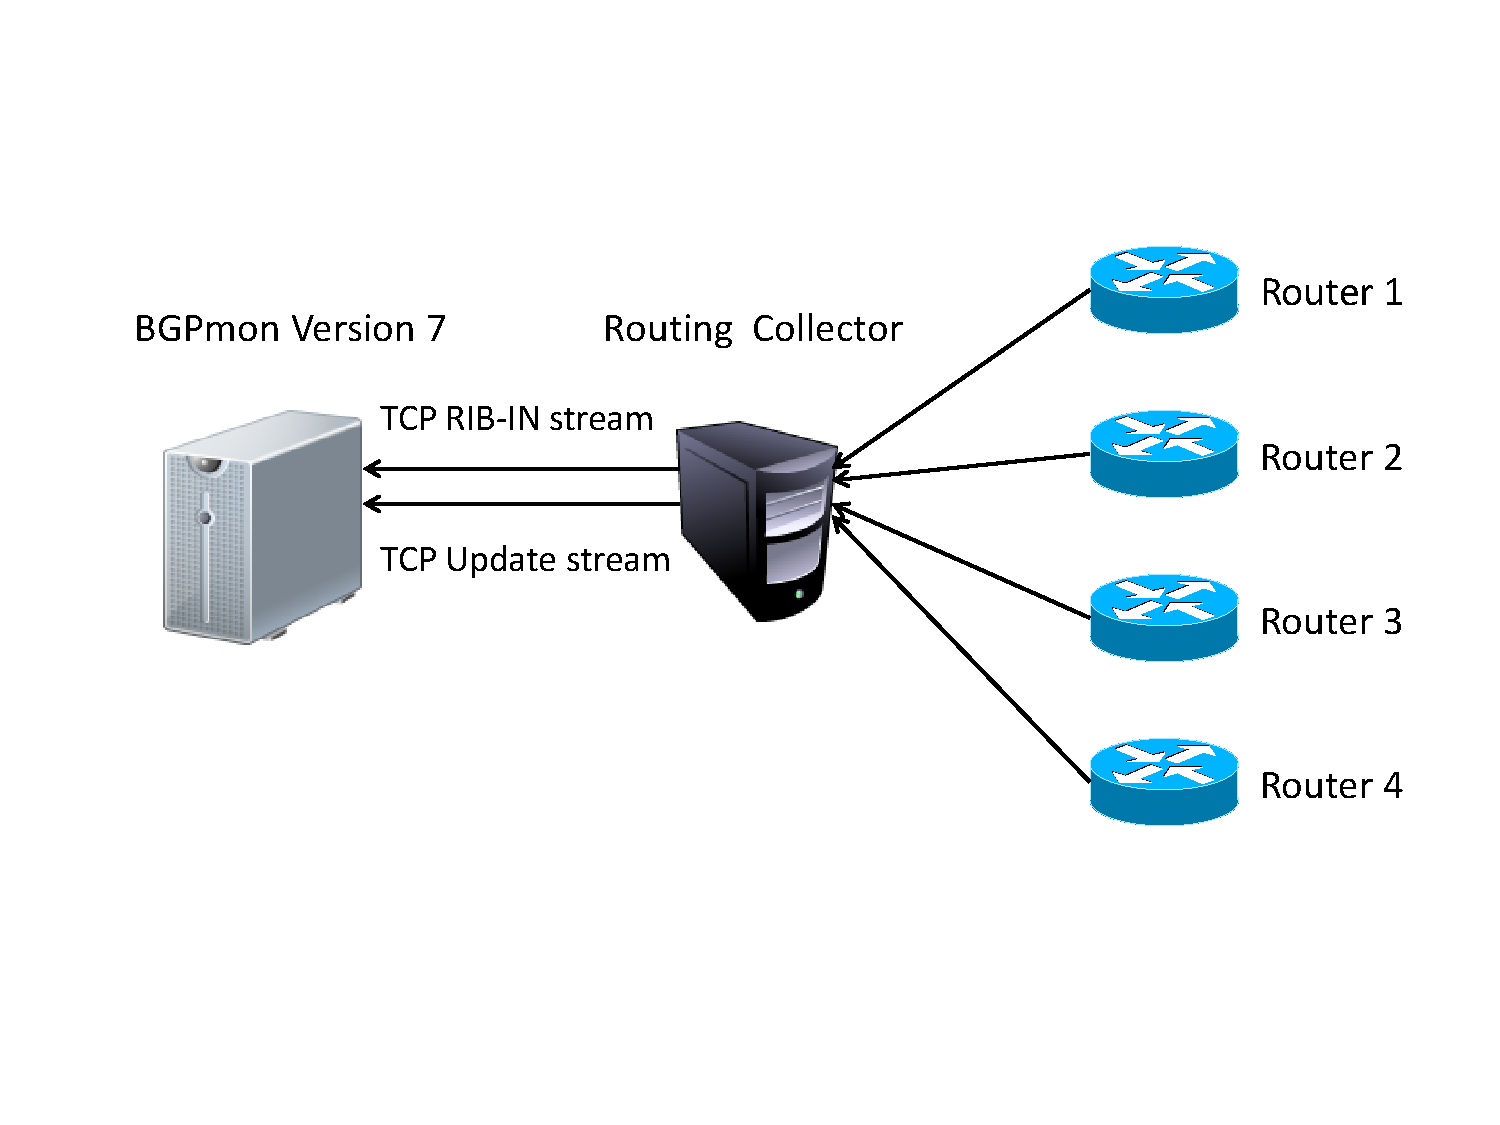
\includegraphics{figs/bgpmon-quagga.pdf}}
\caption{BGPmon and Routing Collector}
\label{fig:routingcollector}
\end{figure*}

In our design, we develop a patch to RC to support MRT format\cite{mrt}. Patch adds new functions to the Routing Collector to sends MRT messages (which contains updates or RIB-IN table) via TCP connection. Figure \ref{fig:routingcollector} shows example, where Routing Collector has multiple TCP sessions to Router 1-4 and just 2 TCP connections to BGPmon.  


% The Routing Collector has multiple BGP peering sessions with Routers 1-4. In our design, Routing Collector creates and uses multiple TCP connections to BGPmon. RC can create TCP session to send MRT update messages or to send MRT RIB-IN tables. This design was chosen because of MRT message format. Every header in MRT message contains each of router's IP address, port number and AS number. Using MRT header message, BGPmon can distinguish BGP messages originated from different RC's peers.

%in particular,   we are using this text to discuss our approach with a competing solution that could obsolete us.      critical to the discussion are the problems in integrating MRT streams.     what are the challenges in doing this?    what are the potential problems?   what is our design decision on the trade-offs.   more specificially
%I don't see a clear explanation of why the RC should send both a RIB table and updates.
%I don't see any example of how update streams and RIB tables are synchronized.

%I don't see any discussion of what happens if the RC sends a second BGP table for say router 1 in your figure.
%I don't see any discussion of why you should send several peers over single session or use one TCP connection for each peer.   for example,  do you send updates from Router 1, 2, 3, and 4 in one TCP session or four?  what are the trade-offs?

Every MRT message has a MRT header and body structure. The header for an update and RIB-IN messages has the same structure: a timestamp (time in seconds, when message originated), a type (type of MRT message), a subtype and a length (length of MRT message without the header). MRT body starts with peer's and RC's IP address, port number and AS number fields.  MRT body for update message contains BGP messages originated by peer, while the MRT body for RIB-IN message has the internal routing table generated by RC. Using MRT header message, BGPmon can distinguish BGP messages originated from different RC's peers.



% describe session structure
%In our implementation, Routing Collector maintains its peer sessions via TCP connection. If RC is using only 2 TCP streams to BGPmon to send routing data, it could create a peer up/down session management problem. For example, if TCP connection is lost to Router 1, RC should erase all BGP attributes and prefixes associated with Router 1. If peer reestablish connection, Routing Collector will create new session structure and start collecting routing data. Session management could be a tough problem for BGPmon - MRT message contains BGPmon is using MRT  message fields (peer IP address, port number and AS number fields) for maintaining "Session ID" structure described in section \ref{sec:peering}. The details of session management logic will be discussed in section \ref{sec:mrt:sessionmanagement}} and \ref{sec:mrt:sessionclosing}.

%describe possible oreder how updates or tables could be received and parsed
In our design, Routing Collector can create multiple TCP connections to BGPmon. Once the TCP connection is established, Routing Collector could send snapshot of MRT RIB-IN messages or MRT update messages. It's important to describe the order how update and table streams are synchronized in BGPmon:
\begin{itemize}
\item{What if first TCP stream contain MRT update messages and second TCP stream contain MRT RIB-IN messages?}
\item{What if first TCP stream contain RIB-IN messages and second TCP stream contain MRT update messages?} 
\end{itemize}

Answer for the first question is simple. For example, Routing Collector sends update message and then RIB-IN table message originated from Route 3. First, BGPmon receives update message and creates a new "Session" structure for Router 3. Then it gets a RIB-IN table for the Router 3. In our design, BGPmon extracts all BGP attributes and prefixes from RIB-IN message and store them in internal BGPmon routing table linked with Router 3 "Session" structure.

Answer for the second question is different: assume that BGPmon receives a RIB-IN table from Router 3 first and update message later. BGPmon will create a new session structure for Router 3 and copy all RIB-IN tables to internal routing table. Future update messages will add or withdraw routes in BGPmon table. 


%BGPmon will store all MRT RIB-IN message in queue buffer. Then, for each of update message, which contain Router 3 IP address, port number and AS number, MRT module will search in queue buffer for same values.
%Second question described correct order of receiving message. Ideally, 

%MRT module will store MRT RIB-IN message in queue buffer. Then, for each of update message, which contain Peer IP address, port number and AS number, MRT module will search in queue buffer for same values. If these values are found in queue buffer, MRT module will extract BGP attributes and prefixes from buffer, create new BMF messages and send them to PeerQueue. Then MRT module will convert update message to BGPmon's internal BMF format and apply this message to PeerQueue. Overall, second question describes the ideal behavior of Routing Collector: first of all, its necessary to send correct picture of routing data (RIB-IN messages). Then Routing Collector should periodically send MRT update messages to change (add or withdraw) BGPmon's internal RIB-IN table.

Also, it's important to mention another issue in this design: What about synchronization of these 2 streams? What should be a time period (timer) between two connections? And can 2 streams overlap? Answer for the last question is yes, they can. To prevent overlapping, BGPmon tracks what stream is processing. If BGPmon processing RIB-IN stream, it will buffer all further update messages and apply them after table extracting is done. Also, is case if BGPmon receiving update stream first and if time period between two connections is too long, we could damage already created BGPmon's routing table. In another case, if time period is too small, two connections could overlap and create a routing mess. In our design, we accept the fact that 5 to 10 minutes period is optimal to use between two streams and this value won't change BGPmon's routing table dramatically.


%I don't see any discussion of how you close a session for a particular session.   for example,   how do you close the session to only router 3.
%I don't see any discussion of what happens if the connection between the  router and the RC fails.    for example,  what happens if RC to router 2 connection fails then restarts.
Another significant design issue is TCP session failure between RC and its peers. For example, BGP peering session between RC and Router 2 fails or closes. Once the session is down,  BGPmon no longer receives updates to the table and the table stored in BGPmon can quickly become out of date.  BGPmon should detect the peering session is now down and delete the routing table for Router 2. For directly connected peers, BGPmon immediately detects the peering session failure following the procedure set out in the BGP standard \cite{bgprfc}. For an indirectly connected peer such as Router 2 in Figure \ref{fig:routingcollector}, the Route Collector has learned the peer is down but this information should be sent to BGPmon. 
% signal part
In order to do that correctly, RC should send a signal to BGPmon that session to Router 2 is failed. Without an explicit signal from the Route Collector, it is difficult for BGPmon to infer that the session failed.
% If RC won't send a signal to BGPmon, Router 2 routing table in BGPmon can become out of date. 
Instead of trying to infer when a session has failed,  the Routing Collector must send an explicit signal indicating the session to Router 2 has failed. In our design, this signal is a MRT RIB-IN message. Header of this message has a Router 2 peering IP address, port and AS number, while message body is empty. When BGPmon receives this message, it should erase all BGP attributes and prefixes associated with Router 2 session structure.
In case, when signal message is lost or did not occur, there might be two problems:
\begin{itemize}
\item{\emph{BGPmon lost a TCP session to Routing Collector:} BGPmon should delete all tables associated with RC peers.}
\item{\emph{Route Collector did not send a signal or signal was incorrect:} It could be a complex problem for BGPmon to keep all routing data in current state. If Route 2 connection to RC failed, RC won't be able to send BGPmon any update message.}
\end{itemize}

The important design issue here is how to manage data from peer which reestablished connection with Routing Collector. For example, Routing Collecter restarts BGP session with Router 4, BGPmon will start receiving routing data from RC. First of all RC should provide a RIB-IN table from Router 4. It couldn't be done immediately after tcp connection is opened. Routing Collector needs to create its own RIB-IN table. After that, RC must send table to BGPmon. Secondly, all BGP update message originated from Router 4 should be send to BGPmon after the first step is done. 

In our design, as described previously, BGPmon is able to receive RIB-IN table multiple times from the same Router 4. It could happen when TCP connection between RC and Router 4 fails and restarts again.  In order to have correct routing picture in BGPmon, we assume that every time when BGPmon receives RIB-IN table, it should erase all BGP attributes and prefixes associated with "Session" structure (in our example, Router 4 "Session" structure) from its table and apply the new table by extracting data from MRT RIB-IN message. 

Moreover, we should discuss another important issue is how Routing Collector manage BGP peers with different AS number (ASN) lengths in BGP attributes\cite{bgprfc}. Also, we will discuss problems which could occur and trade-offs in our design. Following the topology example shown in Figure \ref{fig:routingcollector}, lets assume that Router 1 and Router 2 are using 2-byte ASNs, while Router 3 and 4 - 4-byte ASNs. When Routing Collector establishes BGP peering session with the Routers, each of Routers will send BGP capabilities to indicate what AS length they support. In particular example, Routers 1,2 will send BGP capabilities that both of them support 2-byte ASN length and Router 3,4 - 4-byte ASN length. In this case, Routing Collector should organize routing table properly for each of the peers. There could be two possible solutions how to handle peers with different ASN lengths:
\begin{itemize}
\item{Routing Collector could maintain a routing table with different AS number lengths for each of peers.}
\item{Routing Collector could use 4-byte AS number length as default for all peers.}
\end{itemize}

Fist solution looks reasonable - Routing Collector need to have key parameter, which will store AS number length value for each of peering Routers. This assumption makes routing table not perfectly organized, for each of peers, there will be different AS path length and different peer session structure. In terms of future Internet development and simplicity of adding new features to the routing protocols, we think that Routing Collector should use a 4-byte AS number length as default: RC should not worry about peer AS number length. It could use 4-byte length fields to store 2-byte or 4-byte long AS numbers. 

If Routing Collector is using 4-byte ASN length a default ASN length for all of peers, it creates other problems for BGPmon: Routing Collector could send routing table to BGPmon in 4 byte AS number length format, while update messages from peers could be 2-byte long. In example shown in Figure \ref{fig:routingcollector}, Routing Collector could send RIB-IN tables from Router 1, which is using 2-byte AS length, in 4-byte format. Moreover, Routing Collector will provide further update message in 2-byte format from Router 2. This problem might create a mess in BGPmon's routing table. In order to eliminate following issues, we made few important changes to our design: 
\begin{itemize}
\item{\emph{If, Routing Collector sends RIB-IN table in 4-byte format from Router 1 and further update messages from the same routers are 2-byte long, BGPmon should convert Router 2's entire routing table to use 2-byte ASN length.}} 
\item{\emph{If, Routing Collector sends RIB-IN table in 4-byte format from Router 1 and further update messages from the same routers are 4-byte long, BGPmon won't add any changes to its routing table. }} 
\item{\emph{If, Routing Collector sends RIB-IN table in 2-byte format from Router 1 and further update messages from the same routers are 2-byte long, BGPmon won't add any changes to its routing table.}}
\item{\emph{If, Routing Collector sends RIB-IN table in 2-byte format from Router 1 and further update messages from the same routers are 4-byte long, BGPmon print a error to log.}}
\end{itemize}











% Route Collector should send an empty RIB-IN message for Router 2. If connection between Router 2 and Route Collector restarts, RC should send 

% For example, if TCP connection is lost between Router 3 and RC. In our design, RC will send empty RIB-IN tale only for Router 3 
%Routing Collector maintains TCP session with its peers and MRT message format does not allow us to know, when TCP connection fails or closes between Routing Collector and peer. In our design, instead of adding and keep tracking timeout value for each of created "SessionID's", 

%If TCP connection between the Router 2 and the RC fails, RC sends RIB-IN message with empty routing table of Router 2. At BGPmon side, MRT module will erase all BGP attributes and prefixes associated with this peer. If Routing Collector restarts connection with a Router 2, it sends newly created MRT RIB-IN and update messages to BGPmon. Further, MRT module will create new "Session" structure with BGP attributes and prefixes. 

%If TCP connection restarts, RC will recreate its own routing table and send 

%ample,  what happens if RC to router 2 connection fails then restarts.

%In case if Routing Collectors sends entire MRT RIB-IN messages periodically, BGPmon MRT module will reset all routing tables of "SessionID's" associated with Routing Collector's data and create new "Session" structures.

 
%We added a timeout value for each of created sessionID's. If no MRT update message arrived during the timeout period, %we assume that TCP session fails and Session Close function should be called. If Routing Collector reestablish %connection with its peer, new MRT RIB-IN and update message should be forwarded to BGPmon.

%describe possible situations with number of tcp connections: 



%Routing Collector sends MRT data in different ways: 

%It's important to mention about the order of receiving update and RIB-IN messages: first, MRT module receives RIB-IN message snapshot from RC and then update %messages only to add or withdraw routing changes to BGPmon's internal RIB-IN routing database. Future RC RIB-IN messages should be discarded.
\subsubsection{BGPmon MRT module overview}
BGPmon MRT module supports 2 types of MRT messages (see \cite{mrt}):
\begin{itemize}
\item{\emph{Update message:} This message has a header structure with "BGP4MP" type and "BGP4MP\_MESSAGE" or "BGP4MP\_MESSAGE\_ AS4" subtype and message body with  BGP attributes and prefixes. }
\item{\emph{RIB-IN message:} This messages has header structure with "TABLE\_DUMP\_V2" type and contains all routing data from Routing Collector (RC).}
\end{itemize}

Messages with other MRT header types (for example OSPF, ISIS) are ignored and error message will appear in log file or stdio output.



\subsubsection{Processing MRT updates}
MRT update message, received from Routing Collector, has following fields:
\begin{itemize}
\item{\emph {Peer address:} Peer IPv4 or IPv6 address}
\item{\emph {Local address:} RC IPv4 or IPv6 address}
\item{\emph {Peer AS:} Peer AS number, could be 2-bytes or 4-bytes length}
\item{\emph {Local AS:} RC AS number, could be 2-bytes or 4-bytes length}
\item{\emph {BGP Message:} BGP Message with attributes and prefixes}
\end{itemize}
MRT module parses update message following MRT draft specification and converts it to internal BMF BGPmon message. Then new BMF message applied to PeerQueue.

\subsubsection{Processing MRT RIB-IN tables}
Routing Collector sends RIB-IN table message only once after successful TCP connection. RIB-IN messages have MRT header structure with "TABLE\_DUMP\_V2" type and current timestamp. Main body message contains list of all peer clients connected to Routing Collector and their BGP attributes and prefixes. BGPmon MRT module parses this message, creates and sends new BMF message to PeerQueue.

\subsubsection{Session Management}
\label{sec:mrt:sessionmanagement}
When Routing Collector establishes TCP connection to BGPmon and new messages (update or RIB-IN table) arrives, MRT module makes the following checks based on first arrived message:
\begin{itemize}
\item{\emph{First message is RIB-IN message:} MRT module creates RIB-IN queue buffer and copy all RIB-IN messages to the buffer.}
\item{\emph{First message is update message:} MRT module creates new Session structure with sessionID (based on Peer IP address, port and AS number), searches through the RIB-IN queue buffer for BGP attributes and prefixes associated with sessionID. Then MRT module creates new BMF messages and sends them to PeerQueue. }
\end{itemize}

\subsubsection{Session Closing}
\label{sec:mrt:sessionclosing}
RC's TCP connection sends multiple update messages from its peers, MRT module keeps track of all SessionIDs created with particular RC. If RC's connection fails or closes, MRT module will:
\begin{itemize}
\item{{Change Label Action:} Change all states of previously created Session IDs to "stateError". }
\item{{Delete Attributes:} Delete all BGP attributes and prefixes from BGPmon internal RIB-IN table. }
\end{itemize}

\subsubsection{2 bytes and 4 bytes AS length format}
BGPmon MRT module supports update and RIB-IN messages containing 2-bytes or 4-bytes length AS Path. Current software implementation of Routing Collectors could send updates or RIB-IN messages using different format. Based on received data, MRT module makes following changes to ASPath associated with SessionID structure:
\begin{itemize}
\item{\emph{First message is RIB-IN and has 2 byte ASN}}
	\begin{itemize}
		\item{\emph{Second message is update and has 2 bytes ASN:} MRT module will process this update message without any changes}
		\item{\emph{Second message is update and has 4 bytes ASN:} MRT module will print a error and wont process this message}
	\end{itemize}
\item{\emph{First message is RIB-IN and has 4 bytes ASN}}
	\begin{itemize}
		\item{\emph{Second message is update and has 2 bytes ASN:} MRT module will convert internal BGPmon routing table to 2 byte ASPath length}
		\item{\emph{Second message is update and has 4 bytes ASN:} MRT module will process this update message without any changes}
	\end{itemize}
\item{\emph{First message is update and has 2 bytes ASN}}
	\begin{itemize}
		\item{\emph{Second message is RIB-IN and has 2 bytes ASN:} MRT module will process this update message without any changes}
		\item{\emph{Second message is RIB-IN and has 4 bytes ASN:} MRT module will convert ASpath of RIB-IN message to 2 byte ASN }
	\end{itemize}		
\item{\emph{First message is update and has 4 bytes ASN}}
	\begin{itemize}
		\item{\emph{Second message is RIB-IN and has 2 bytes ASN:} MRT module will print error and wont process this message}
		\item{\emph{Second message is RIB-IN and has 4 bytes ASN:} MRT module will process this update message without any changes}
	\end{itemize}	
\end{itemize}

\subsubsection{Corrupted MRT messages}


The MRT module in BGPmon reads fixed-size data chunks from the socket connection and expects well-formatted MRT messages. However, the Routing Collector may send  MRT messages out of order and thus corrupt the internal data structures in BGPmon. To this end, MRT module attempts to recover from corrupted MRT messages.  

\note{BGPmon MRT module is able to recover from corrupted MRT update messages only. Currently there is no recover solution for MRT RIB-IN table messages.
}




The important design decision here is how MRT module finds the next valid MRT update message. The MRT module include two-step procedure for MRT update messages: detection of corrupted messages and recovering from corruption. 

To detect corrupted MRT update message, MRT module validates MRT common header. This procedure includes MRT header values tests. 
\begin{itemize}
\item{MRT module validates the MRT header timestamp. MRT module checks if MRT timestamp value is not bigger than the current timestamp. }
\item{MRT module validates the MRT type and subtype values according to MRT RFC \cite{mrt}. MRT module checks for \emph{TABLE\_DUMP\_V2} and \emph{BGP4MP} types and all inclusive subtypes.}
\item{MRT module validates the MRT header length. In particular, it checks that the MRT message length is not bigger than the max MRT update message (that depends on corresponding MRT type and subtype). }
\end{itemize}

If one of validation tests fail, MRT module start recovering from corrupted MRT update message. This procedure includes following:

\begin{itemize}
\item{Since every MRT update message include BGP message from the wire, the MRT module will try to find valid BGP marker value: 16 bytes of data that contains "0xFF" values. The MRT module reads byte by byte from the socket connection until it finds the BGP marker. }
\item{Once the BGP marker is found, MRT module will try to read 2 bytes of length. However, its important to verify that previous 16 bytes are valid BGP marker. To this end, the MRT module reads one byte of BGP length and checks if the byte value is  not equal to "0xFF" marker value. Upon failure, MRT module continues to read byte by byte from the socket to get the valid BGP message length. Upon success, MRT module will read the second byte of BGP length and merge two bytes together to get the value of BGP message length. }
\item{Lastly, MRT module uses BGP message length to read the remaining number of bytes to get to the end of the BGP message.}
\item{At this point, MRT module expects the start of new MRT update message.}
\end{itemize}



\subsection{Design Philosophy}
The important design decision here is that BGPmon MRT module can receive data from any kind of Routing Collector which supports MRT format specification. For example routing software such as Zebra or Quagga needs a small patch to support MRT format. This patch is available in BGPmon distribution. 



In the design of MRT module, one of important issues is how to handle order of update or RIB-IN messages with 2 or 4 bytes AS Path length. Today's peering routers rarely use 4-bytes AS Path length and they trying to avoid problem with 4 to 2 bytes ASPath conversion. MRT module is using simple solution described in previous subsection.


\section{Labeling Module}
\label{sec:labeling}
Labeling module manages one RIB-IN table associated with a peer if configured and uses the tables to assign labels to updates received from the peer.  In this module, the only configuration is about how to process the BGP updates from peers. It is specified by "labelAction" in peer configuration as shown in Figure \ref{fig:configurationSub}. "labelAction" could be one of these three options:
\begin{itemize}
\item{ \emph{None:} Don't process the updates at all. }
\item{ \emph{RibStore:} Store the updates in RIB-IN tables on a per-peer basis. The peer has its own RIB-IN table if this option is set.}
\item{ \emph{Label:} Store the updates in RIB-IN tables and label the updates based on how they change RIB-IN tables. This option implicitly stores RIB-IN for the peer. }
\end{itemize}
Since the RIB-IN tables are the major memory consumption of BGPmon, one might want to set "labelAction" as "None" if the memory is the major concern. 

Labeling module has a single thread which is a reader of peer queue and a writer of label queue as shown in Figure \ref{fig:architecture}. Main flow has three steps:
\begin{itemize}
\item{ Read the BMF messages from peer queue }
\item{ If the BMF message is a update, then process it based on the "labelAction" configuration. Otherwise, do nothing.}
\item{ Write the processed BMF messages into labeling queue }
\end{itemize}
The detail of main flow logic will be discussed in section \ref{sec:labeling:mainflow}.

\subsection{Data Structure}
Labeling Module uses 2 main data structures(PrefixTable and AttrTable) to maintain the RIB-IN table. As the RIB-IN table is maintained on a per-peer basis, it is natural to make these 2 structures as components of the "Session" structure as we mentioned in section \ref{sec:peering:sessionstructure}.  "PrefixTable" and "AttrTable" are used to store prefixes and attributes in BGP updates respectively. And these 2 tables are inter-linked to make up one RIB-IN table.

\subsubsection{ PrefixTable Structure}
\label{sec:labeling:prefixtable}
In our design it is a hash table that consists of multiple entries. Each entry is a link list of nodes and each node contains a prefix. It has the following six parts.
\begin{itemize}
\item{\emph{prefixCount:} is the number of prefixes are contained in the prefix hash table.}
\item{\emph{tableSize:} is the number of entries in the hash table.}
\item{\emph{occupiedSize:} is the number of occupied entries in the hash table. Occupied entry means it has at least one node. }
\item{\emph{maxNodeCount:} is the max length among all entries in the hash table. The length of one entry indicates how many nodes it contains.}
\item{\emph{maxCollision:} is the max number of nodes one entry is allowed to contain. If one entry contains too many nodes, we need to increase the number of entries in a hash table in order to improve the performance. Basically if maxNodeCount is larger than maxCollision, we need to enlarge the hash table.}
\item{emph{prefixEntries:} is an array of PrefixEntry structures. It contains all the entries of the prefix hash table. For the details of PrefixEntry structure, see Figure \ref{fig:PrefixEntryStruct}.}
\end{itemize}
\begin{figure*}
\centering
\scalebox{0.8}{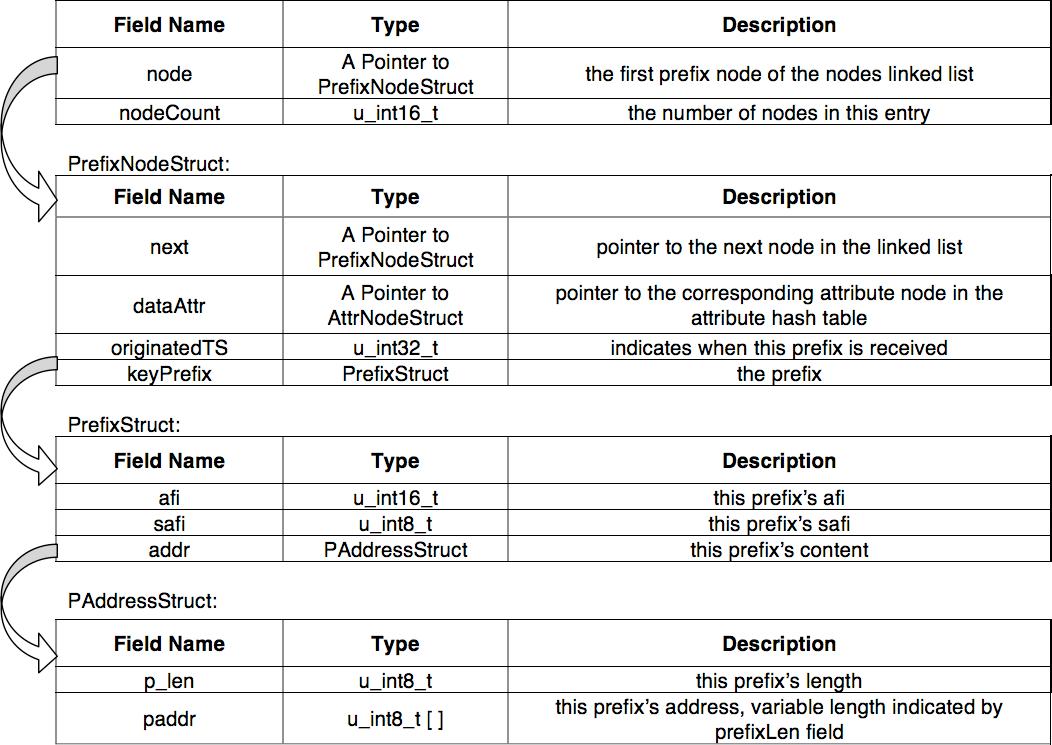
\includegraphics{figs/PrefixEntryStruct.pdf}}
\caption{PrefixEntry Structure}
\label{fig:PrefixEntryStruct}
\end{figure*}
Each prefix in the NLRI of a BGP update will be one node of a particular entry in the prefix table. The index of this entry is calculated by hash value of the prefix. 
2 same prefixes will be hashed to the same entry and stored in the same node.
Because of hash collision, 2 different prefixes could also be hashed to the same entry. But they will be stored in difference nodes of this entry.

\subsubsection{AttributeTable Structure}
\label{sec:labeling:attributetable}
Attribute hash table is similar to the prefix hash table mentioned in the previous section. AttributeTable structure is used to implement a hash table to store the attributes of BGP updates. It has the following six parts.
\begin{itemize}
\item{\emph{attributeCount:} is the number of attributes are contained in the attribute hash table.}
\item{\emph{tableSize:} is the number of entries in the hash table.}
\item{\emph{occupiedSize:} is the number of occupied entries in the hash table. }
\item{\emph{maxNodeCount:} is the max length of all entries in the hash table.}
\item{\emph{maxCollision:} is the max number of nodes one entry is allowed to contain.}
\item{\emph{attrEntries:} is an array of AttrEntry structures. For the details of AttrEntry structure, see Figure \ref{fig:AttributeEntryStruct}.}
\end{itemize}
\begin{figure*}
\centering
\scalebox{1}{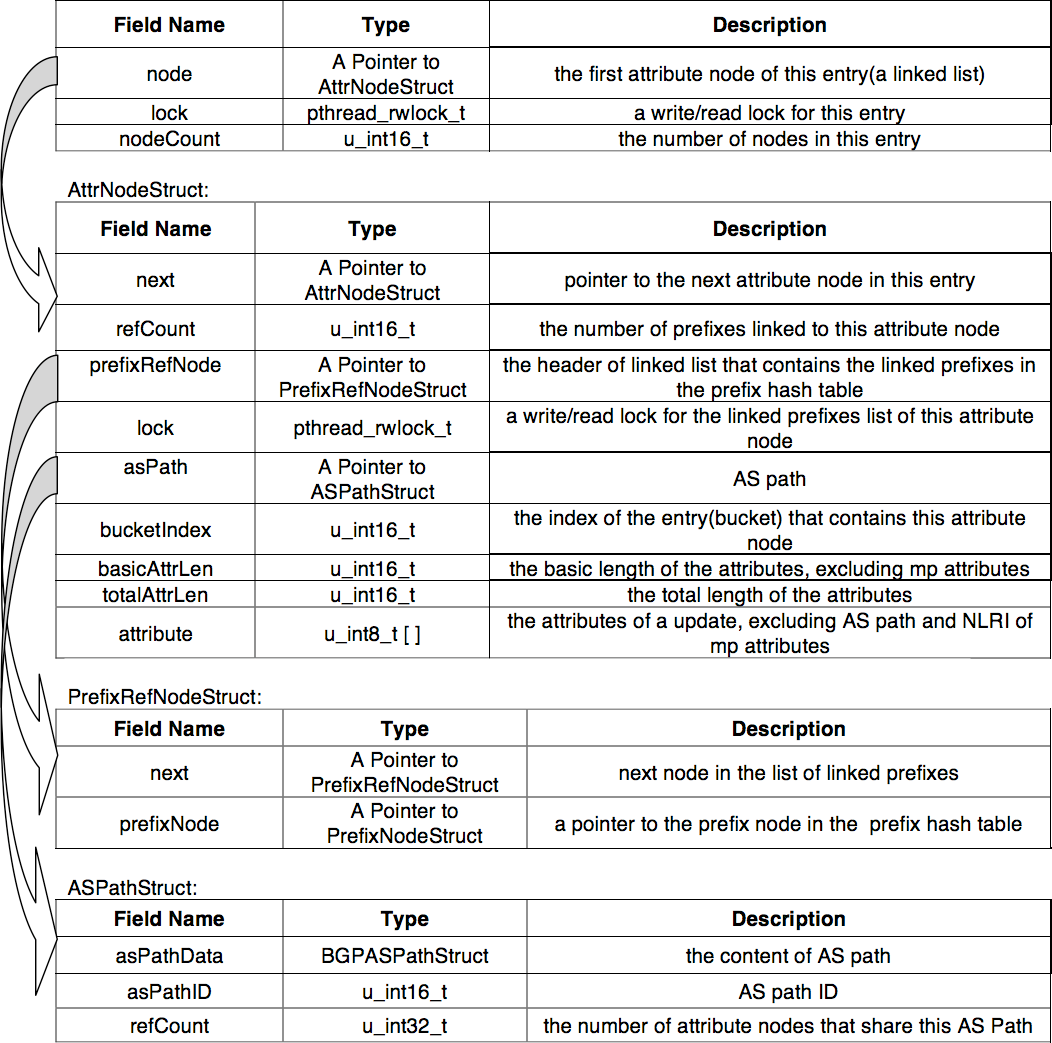
\includegraphics{figs/AttributeEntryStruct.pdf}}
\caption{AttributeEntry Structure}
\label{fig:AttributeEntryStruct}
\end{figure*}
In the attribute table, the attribute set in a BGP update will be stored in one node. And which entry this node belongs to is determined only by the hash value of AS path.
That means if 2 attribute sets have the same AS path, they will be hashed to the same entry. If other attributes of the 2 sets are also same, they will be stored in the same node. 
If 2 attribute sets have the same AS path but other attributes are different, they will still be stored in the same entry but 2 different nodes.  
Note in the case the AS path is only stored once and the 2 different nodes will link to the same AS path.
Again it is possible that  2 attribute sets with different AS paths are hashed to the same entry because of hash collision.

   

\subsection{Main Flow Logic}
\label{sec:labeling:mainflow}
After introducing the data structure, we describe the main flow logic of labeling module here. As we mentioned, labeling module reads the BMF messages from peer queue. For the BMF messages with type other than 2 (see Figure \ref{tab:types}), the labeling module simply writes them into labeling queue without any processing.  For each BMF message with type 2, labeling module processes it as follows:  
\begin{itemize}
\item{If it doesn't contain a BGP update message, simply writes it into labeling queue without any processing.}
\item{If it contains a BGP update message,  extract the session ID from the BMF message. With the sesionID the labeling module finds the peering session structure and checks the 'labelAction' in it (see Figure \ref{fig:configurationSub}).  }
	\begin{itemize}
		\item{If the field 'labelAction' is set to "None", simply writes the BMF message into label queue without any processing.}
		\item{If the field 'labelAction' is set to "RibStore", updates the RIB-IN table of the corresponding peering session and then writes the the BMF message into label queue. In section \ref{sec:labeling:storerib} we will discuss the detail about how to update RIB-IN tables given a BGP update message. }
			\item{If the field 'labelAction' is set to "label", updates the RIB-IN table of the corresponding peering session and labels this BMF message. Specifically, one label for each prefix in NLRI will be attached to the BMF message and its message type will be changed to 3. Finally the new BMF message with type 3 will be written into label queue. In section \ref{sec:labeling:label} we will discuss the detail about how to label a BGP update message.}
	\end{itemize}
\end{itemize}

\subsection{Store RIB-IN Tables}
\label{sec:labeling:storerib}
The labeling module stores RIB-IN tables on a per-peer basis. For each incoming BGP update message from a peer, the labeling module stores it in the peer's RIB-IN table as follows:
\begin{enumerate}
	\item{Parse the BGP update message into the following components:}
	\begin{itemize}
		\item{IPv4 unicast reachable NLRI and unreach NLRI}
		\item{multiple protocol(mp) reachable NLRI and unreach NLRI}
		\item{the attribute set excluding AS path, mp unreachable attributes and NLRI of mp reachable attributes}
		\item{AS path}
	\end{itemize}
	
	\item{Hash the AS path and find the entry in the attribute table based on the hash value. Then check each node of this entry against the AS path and attribute set from above as follows:}
	\begin{itemize}
		\item{If the current node's AS path and attribute set are the same, return this attribute node.}
		\item{If the current node's AS path is same but attribute set is not, return a new created attribute node that has the new attribute set and is linked to the existing AS path. Recall the same AS path shared by multiple nodes is only stored once.}
	\end{itemize}
	\item{If none of the nodes matches the above 2 rules, return a new created attribute node with the new AS path and attribute set.}
		
	\item{Extract all prefixes from IPv4 unicast reachable NLRI and mp reachable NLRI. Each prefix is processed as follows: }
	\begin{itemize}
		\item{If there is a existing prefix node which contains the same prefix content such as such as afi, safi, mask length and address in the prefix hash table:}
		\begin{itemize}
			\item{If the existing prefix node's linked attribute node('dataAttr' field in Figure\ref{fig:PrefixEntryStruct}) is same as the attribute node returned from step 2, do nothing.}			\item{Otherwise:}
			\begin{itemize}
				\item{Delete this prefix node from its current attribute node's linked prefix nodes list. If there isn't any prefix node linked to this attribute node after this deletion, remove this attribute node from the attribute hash table.}
			\item{Add this prefix node to the linked prefix nodes list in the attribute node returned from step 2.}
			\end{itemize} 	
		\end{itemize}
		\item{Otherwise:}
		\begin{itemize}
			\item{Create a prefix node(PrefixNodeStruct, see Figure\ref{fig:PrefixEntryStruct}) based on the prefix's content.}
			\item{The created prefix node is placed into an entry(PrefixEntryStruct, see Figure\ref{fig:PrefixEntryStruct}) in the prefix hash table based on the hash value of the prefix's content.} 			\item{Update its linked attribute node field('dataAttr' field in Figure\ref{fig:PrefixEntryStruct} with the attribute node returned from step 2. }
			\item{As each attribute node maintains a list of all linked prefix nodes, we also need to add this new created prefix node to that list of the attribute node returned from step 2}
		\end{itemize}
	\end{itemize}
	
	\item{Extract all prefixes from the IPv4 unicast unreachable NLRI and multiprotocol unreachable NLRI. Each prefix is processed as follows:}
	\begin{itemize}
		\item{If there is a existing prefix node which contains the same prefix content such as such as afi, safi, mask length and address in the prefix hash table:}
		\begin{itemize}
			\item{Delete this prefix node from its corresponding attribute node's linked prefix nodes list. If there isn't any prefix node linked to this attribute node after this deletion, remove this attribute node from the attribute hash table.}
			\item{Remove this prefix node from the prefix hash table.} 		\end{itemize} 					
		\item{Otherwise: Do nothing.}
	\end{itemize}		
\end{enumerate}


\subsection{Labels the BGP updates}
\label{sec:labeling:label}
The labeling module labels all the prefixes in a BGP update message base on how they change RIB-IN tables. More specifically, the label classifies the prefixes into six categories: 'new announcement' versus 'duplicate announcement', 'same path' versus 'different path' and 'withdraw' versus 'duplicate withdrawal'. In BGP one update consists of multiple prefixes which share the same set of attributes and these prefixes might change the RIB-IN tables in different ways. As a result, the multiple prefixes in one BGP updates have to be labeled separately. That's why labeling has to be done on a per-prefix basis, not a per-update basis.

Labeling is done as follows:
\begin{enumerate}
	\item{Return a existing or new created attribute node according the step 1 and 2 in the preview subsection. }
	\item{Extract all prefixes from IPv4 unicast reachable NLRI and multiprotocol reachable NLRI. Each prefix is labeled as follows: }
	\begin{itemize}
		\item{If there is a existing prefix node which contains the same prefix content such as such as afi, safi, mask length and address in the prefix hash table:}
		\begin{itemize}
			\item{If the existing prefix node's linked attribute node ('attributeNode' field in Figure\ref{fig:PrefixEntryStruct} is same as the attribute node return from step 1, label it as 'duplicate announcement'.}			\item{Otherwise, compare the 'AS Path' in this prefix node's current linked attribute node to the 'AS Path' in the attribute node returned from step 1. }
			\begin{itemize}
				\item{If they are same, label it as 'same path'. }				\item{Otherwise, label it as 'different path'. }
			\end{itemize} 	
		\end{itemize}			    
		\item{Otherwise, label it as 'new announcement'. }
	\end{itemize}
	
	\item{Extract the IPv4 unicast unreachable NLRI and multiprotocol unreachable NLRI. Each prefix is labeled as follows:}
	\begin{itemize}
		\item{If there is a existing prefix node which contains the same prefix content such as such as afi, safi, mask length and address in the prefix hash table, label it as 'withdraw'}		
			\item{Otherwise:  label it as 'duplicate withdraw'.}
	\end{itemize}
\end{enumerate}
	
\subsection{Design Philosophy}
The first design issue here is how to organize a RIB table in memory. Logically a RIB table can be viewed as prefixes and attributes that are interlinked together. And another observation is that a set of attributes is typically shared by multiple prefixes as they are received in one BGP update.  Based on these observations. we decided to store a RIB by using 2 interlinked hash tables: prefix hash table and attribute hash table.
As we discussed in subsecions \ref{sec:labeling:prefixtable} and \ref{sec:labeling:attributetable}, these 2 hash tables has the same structure in a high level. Specifically both of them consists of multiple entries and each entry is a linked list that has multiple nodes. In the prefix hash table each node represents a prefix and in attribute hash table each node holds a set of attributes. And the prefixes and the set of attributes are linked together if they are received in the same BGP update. Note one prefix node representing a single prefix can only be linked to one attribute node holding a set of attributes. But one attribute node could be linked to multiple prefix nodes. In other words, the relationship between prefix node and attribute node is many to one.

The second design issue is how to store the prefixes and the set of attributes in a BGP update efficiently. For a prefix it is straightforward to hash the prefix to an entry(bucket) in the prefix hash table. Then all the nodes of this entry are checked in order to know if this prefix is existing or not. For the set of attributes, we have 2 options here:
	\begin{itemize}
		\item{\emph{Option1: }Hash the entire set of attributes to an entry of attribute hash table.}		
		\item{\emph{Option2: }Extract the AS path form the set of attributes and then hash the AS path to find an entry for the set of attributes.}
	\end{itemize}
Each option has its own pros and cons. Option1 basically hashes each unique set of attributes to a different entry(bucket) if ignoring the hash collision. That will make the attribute hash table too long in terms of the number of entries.
In option2 each set of attributes is assigned to a entry based on the hash value of its AS path. The implication is that all sets of attributes with the same AS path will be assigned to the same entry. As a result, option2 will take fewer entries than needed by option1. But each entry will have more nodes in option2 than option1. So it is a tradeoff between the number of entries and the length of entries.

But besides that option2 is better in comparing the AS paths in 2 sets of attributes. In option2 2 sets of attributes that have different AS paths must be assigned to the different entry. But  2 sets of attributes assigned to the same entry don't necessarily have the same AS path because of hash collision. So when attribute node gets created we tag its AS path with ID in order to differentiate the different AS paths that are assigned to the same entry because of hash collision. As a result, we can compare the AS paths in 2 sets of attributes as follows:
	\begin{itemize}
		\item{If they are assigned to different entries, we know they have different AS paths.}
		     \item{If they are assigned to the same entry, continue to compare their AS Paths' IDs.}
		\begin{itemize}
			\item{If they are the same, we know they have the same AS path.}			
				\item{Otherwise, we know they have different AS paths.}
		\end{itemize}
	\end{itemize}
Contrast to option2, comparing the AS paths in 2 sets of attributes would be more complex in option1 because one first needs to extract the 2 AS paths from them then compare the 2 AS paths in bitwise. That could be a big flaw of option1 as this operation is done for every receiving prefix in BGPmon.

Another advantage of option2 is that all the sets of attributes have the same AS path will share the same AS path structure in memory. In option1 each set of attributes stores the AS path respectively even some of them have the same AS path. So option2 is also better in terms of memory consumption.
Based on all of these, we decided to use option2 in our current design.
 
The last design issue here is about configuration changes. As we mentioned, the only related configure item here is "labelAction" which has 3 values: None, RibStore and Label. All the possible changes are listed:
\begin{itemize}
\item{If "labelAction" changes from Label to RibStore, nothing needs to be done. The labeling module will automatically turn off the labeling fucntion.}
\item{If "labelAction" changes from RibStore to Label, nothing needs to be done. The labeling module will automatically turn on the labeling fucntion.}
\item{If "labelAction" changes from RibStore to None, the RIB table needs to be freed.}
\item{If "labelAction" changes from Label to None, the RIB table needs to be freed.} 
\item{If "labelAction" changes from None to Label, this change cannot be applied immediately. If we apply this change immediately, the labeling will misbehave as we don't have the RIB. For instance, right after the change all the updates labelled as 'new announcement' are actually not new. } 
\item{If "labelAction" changes from None to RibStore,  this change cannot be applied immediately either. If we start to store RIB immediately and right after that user further changes it from RibStore to Label, we will run into the same problem as above. } 
\end{itemize}
The only way to make the last 2 changes applied is to reset the session. When a new session starts, the changes will be applied automatically and labeling will behave correctly.

\section{Periodic Event Handling Module}
\label{sec:periodic}
Periodic event Handling Module(periodic module in short) manages periodic events such as route refresh requests and periodic status messages.
This module has two threads:
\begin{itemize}
%\item{Periodically writes sessions status trigger message (type 3) into label queue if configured.}
\item{\emph{Periodic Status Messages Thread:} It periodically writes session status messages(BMF type 5), queues status messages(BMF type 6) and chains status messages(BMF type 7) into label queue if configured.}
\item{\emph{Route Refresh Request Thread:} It centralized schedules and executes the route refreshes for all the peers if configured. For each peer, there are two possibilities. }
	\begin{itemize}
		\item{If this peer supports route refresh, periodic module will notify peering module to send route refresh request to the peer.}
		\item{If this peer doesn't support route refresh, periodic module will simulate route refresh by sending local stored RIB-IN out.}
	\end{itemize}
\end{itemize}

The main data structure of periodic event handling module has five fields:
\begin{itemize}
%\item{\emph{sessionsStatusTriggerInt:} It indicates the interval of sending sessions status trigger messages. It is set by configuration module and read by periodic module. }
\item{\emph{StatusMessageInterval:} It indicates the interval of sending periodic status messages for peering sessions, queues and chains. It is configured by user. }
%\item{\emph{sessionsStatusTriggerTimer:} It indicates when is the next time to send sessions status trigger message. It is set and read by periodic module. }
\item{\emph{RouteRefreshInterval:} It indicates the interval of requesting route refresh for every peer that is configured for route refresh. It is configured by user }

%\item{\emph{sessions:} It is a pointer to an array of session structures for all the peers. It is set by configuration module and read by periodic module.}
%\item{\emph{RLs:} It is a pointer to an array of rib and labeling structures for all the peers. It is set by configuration module and read by periodic module.}
\item{\emph{labelQueueWriter:} It is used to write messages into the label queue.}
\item{\emph{shutDownFlag:} It is used to signal periodic module to exit. Specifically both threads keep checking this flag, they will quit if it becomes TRUE.}
\end{itemize}
%\item{\emph{routeRefreshes:} It is a array of RouteRefresh structures. Each session(peer) is attached with one RouteRefresh structure. Each RouteRefresh consists of three field.}
%	\begin{itemize} 
%		\item{\emph{sessionID:} It is a 16 bit session identification. It is set by configuration module and read by periodic module.}
%		\item{\emph{routeRefreshInt:} It indicates the interval of route refresh for this session(peer). It is set by configuration module and read by periodic module.}
%		\item{\emph{routeRefreshTimer:} It indicates the next scheduled route refresh time. It is only used by periodic module. }
%	\end{itemize}
%\end{itemize}
%For the details of this structure, see Figure\ref{fig:PeriodicModuleStruct}.
%\begin{figure*}
%\centering
%\scalebox{1}{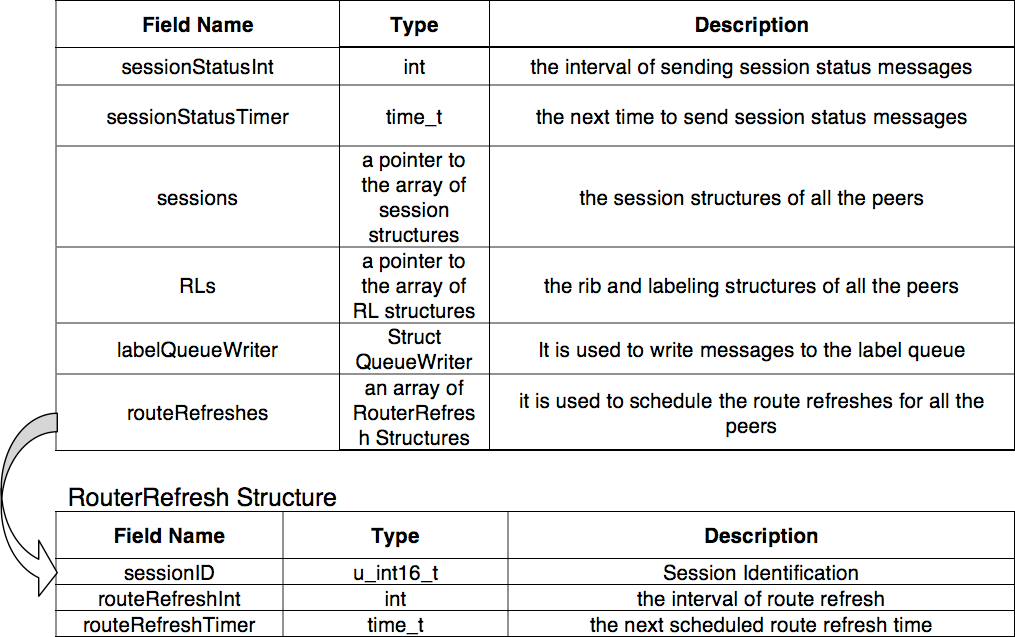
\includegraphics{figs/PeriodicModuleStruct.pdf}}
%\caption{Data Structure of Periodic Event Handling Module}
%\label{fig:PeriodicModuleStruct}
%\end{figure*}
Next we will discuss the detail of the two threads.

\subsection{Periodic Status Messages Thread}
%\subsubsection{ Session Status Message Format}
This thread writes one status message for each peering session, one status message fro all queues and one status message for all chains into the label queue every 'StatusMessageInterval' interval.  Peering session status message (BMF type 5) only includes a session ID instead of including the detail information. Queues' status message(BMF type 6) and chains' status message(BMF type 7) are not associated with a particular peering session.

Then when XML module reads a session status message from label queue, it will extract the session ID from it and retrieve the detail information based on the session ID. Finally the detail information of a peering session will be converted to XML and write into a XML queue. The detail is built from peering session structure( see section \ref{sec:peering:sessionstructure}).  More specifically, it consists of the follow fields:
%\begin{itemize}
%\item{\emph{fsm\_state:} is the current state of FSM that could be one of the six values: Idle, Connect, Active, OpenSent, OpenConfirm and Etablished.  }
%\item{\emph{last\_action:} is a timestamp that indicates when the last action of a peering session is.}
%\item{\emph{establish\_time:} is a timestamp that indicates when the peering session gets established. }
%\item{\emph{message\_rcvd:} is the number of received BGP messages. }
%\item{\emph{prefix\_count:} is the number of prefixes in RIB-IN table. }
%\item{\emph{attribute\_count:} is the number of unique attributes sets in RIB-IN table. }
%\item{\emph{connect\_retry\_count:} is the number of times to retry a tcp connection. }
%\item{\emph{session\_down\_count:} is the number of times BGP session goes down. }
%\item{\emph{session\_last\_down:} is a timestamp that indicated when BGP session went down last time. }
%\end{itemize}
When XML module reads a queues status message from label queue, it will ignore the session ID from it and retrieve the status information all queues. Finally the status information of all peers will be converted to XML and write into a XML queue. Similarly when XML module reads a chains status message from label queue, it will ignore the session ID from it and retrieve the status information all chains.
For the XML format of these periodic status messages, please refer to the XML specification.

%\begin{itemize}
%\item{\emph{FSM Info:} It contains 'state', 'keepaliveInt', 'holdTime', 'routeRefreshType' from FSM substructure in session structure and 'routerRefreshInt' from RouteRefresh Structure. }
%\item{\emph{Session Stats:} It contains all the fields from statistics substructure in session structure.}
%\item{\emph{RIB and Label Stats:} It contains all the stats related fields from RL structure.}
%\end{itemize}
%For the details of session status message, see Figure\ref{fig:SessionStatusStruct}.
%\begin{figure*}
%\centering
%\scalebox{1}{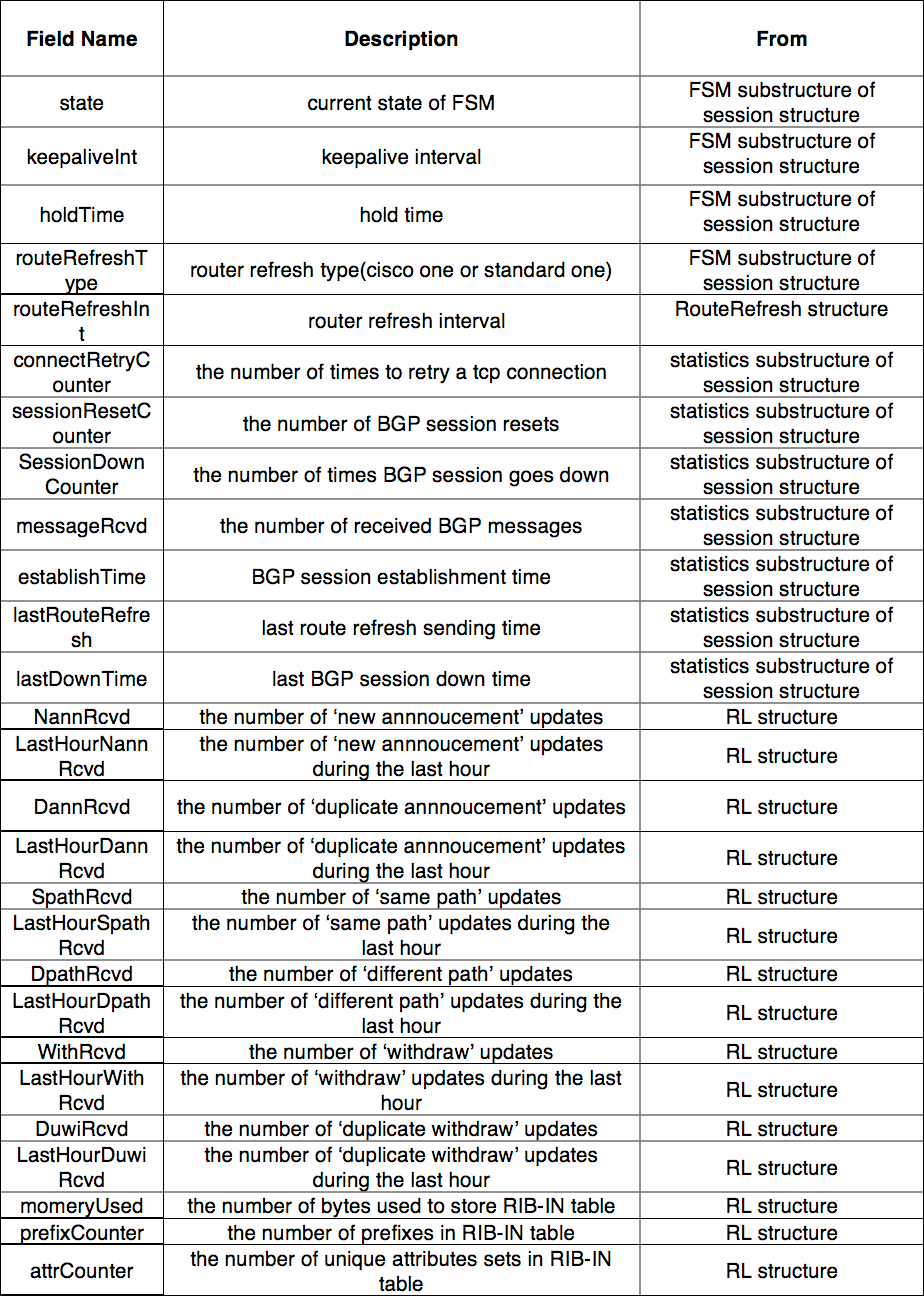
\includegraphics{figs/SessionStatusStruct.pdf}}
%\caption{Data Field of Session Status Message}
%\label{fig:SessionStatusStruct}
%\end{figure*}

%\subsubsection{Send Session Status Messages}

%The 'sessionStatusTimer' field works as a timer to send session status messages for all the peers. When it is timed out, the periodic module will first retrieve all the sessions based on the 'sessions' field in its data structure. Then for each session, the periodic module does the following:
%\begin{itemize}
%\item{Based on its session ID, locate the corresponding RL structure from 'RLs' field in its main data strcutrure.}
%\item{Based on its session ID, locate the corresponding RouteRefresh structure from 'routeRefreshes' field in its main data strcutrure.}
%\item{Create the session status message based on the session ID and current time.}
%\item{Build the data field of created session status message based on the session structure, RL structure and RouteRefresh Structure as we mentioned in the previous subsection. }
%\item{Write this session status message into label queue.}
%\end{itemize}
%If there are several hundreds of sessions, we might want to spread all the session status messages over time evenly in order to avoid a sudden spike in the label queue.

\subsection{Route Refresh Request Thread}
%In our design, the route refreshes for all the peers spread over time evenly in order to avoid overwhelming the queues. 
This thread distributes the route refresh requests for all established peering session evenly over time in order to prevent the queues being overwhelmed.  
%One possible algorithm: 
%\begin{itemize}
%\item{Divide a particular period into several slots. For example, divide 1 hour into 20 slots.}
%\item{Based on the 'routeRefreshes' field, we can know the route refresh interval for each peer. For each peer, we try to find a slot for its first route refresh. }
%\item{If a slot is scheduled by another peer, try the next slot. If all the slots are filled, use the slot with fewest peers. So multiple peers may be scheduled in the same slot.}
%\item{Execute the nearest scheduled route refresh and find a new slot for this peer's next route refresh using the same rules mentioned in the previous step. }
%\end{itemize}

%\subsection{Execute a Scheduled Route Refresh}
If a route refresh request is for one peer that supports route refresh, the periodic module just needs to notify peering module to issue a route refresh request message. Otherwise the periodic module has to simulate a route refresh by sending out this peer's local RIB-IN. The detail of handling the route refresh request for a establish peering session is as follows:
\begin{itemize}
%\item{ Look up the array of session structures which is pointed by 'sessions' field and find this peer's session structure based on its session ID.}
\item{ Check if route refresh is enabled for this session. If not, do nothing. Otherwise, continue. }
\item{ Check the 'routeRefreshType' field of session structure( see section \ref{sec:peering:sessionstructure})..}
	\begin{itemize}
 	\item{if it is 0, that means this peer doesn't support route refresh. The periodic module needs to send out this peer's RIB-IN table as follows:}
			\begin{itemize}
				%\item{Look up the array of RL structures which is pointed by 'RLs' field and find this peer's RL structure based on its session ID.}
				\item{The 'prefixTable' and 'attributeTable' fields of the found RL structure compose this peer's RIB-IN. For each node in the attribute table, do the following things:}
					\begin{itemize}
						\item{Find all the related prefix nodes in the prefix table. }
						\item{Build a BMF message(type 4) that contains a BGP update that is built based on the attribute node and all related prefix nodes.}						
								\item{Write this BMF message into label queue.}
					\end{itemize}	
			\end{itemize}
	  \item{Otherwise, that means this peer supports route refresh. The periodic module just needs to set the 'routeRefreshFlag' field of session structure to TRUE in order to signal the peering module to send out route refresh request to the peer.}
 	\end{itemize}
\end{itemize}

 \subsection{Design Philosophy}
 Actually in the previous design we used to put the logic of sending route refresh requests and periodic status messages in the peering module. 
 More specifically each peering thread decides when to send its own route refresh requests and periodic status messages. 
 But it turns out we lost the ability to schedule these events from a global view. Specially for route refresh requests, it is important to schedule them carefully as each of them will trigger hundreds of thousands of messages that could be a  big burden for the entire system. If all the peers' route refresh request are scheduled at the same time, the queues in BGPmon might not be able to hold the huge amount of messages trigged by them.
 
In the current design, we have a dedicated module to schedule these events. The route refresh requests of all peers are scheduled evenly over the time based based on "RouteRefreshInterval" and the number of peers in order to prevent the queues from being overwhelmed.  In contrast to route refresh requests, the periodoc status messages of all peers are simply written into the label queue every "StatusMessageInterval" as the size of periodic status message is pretty small. But by decoupling the scheduling from peering module it is easy to plug in some sophisticated scheduling algorithms for the periodic status message as needed.
%\subsection{Dynamic Configuration Change}
%In the periodic event handling module, two parts may be changed dynamically by configuration module.
%\begin{itemize}
%\item{\emph{sessionsStatusTriggerInt:} the interval of sending sessions status trigger messages.}
%\item{\emph{routeRefreshInt:} the router refresh interval of each peer.}
%\end{itemize}
%These configuration changes can be automatically adopted when the periodic module sets the time for the next sessions status trigger message and route refresh.
\section{XML Generation Module}
\label{sec:xml}

%The XML thread simply copies from the label queue to the xml queue for processing by the clients.
The XML generation module manages the conversion of all BGPmon received and generated messages into XML. It has one single thread which consists of three main steps. 
\begin{itemize}
\item{It reads messages from the label queue. These messages can be any of all eight types in Figure \ref{tab:types}.}
\item{It converts all types of messages into XML format according to our XML specification. }
\item{It writes messages in XML format to the XML queue for processing by the client threads.}
\end{itemize}

%The main data structure of  XML generation module only consists of two fields.
%\begin{itemize}
%%\item{\emph{expandModeFlag}: It is a 0 or 1 flag. If it is set to 0, the XML generation module will work in normal mode. If it is set to 1, it will work in expand model. We will discuss these two modes later in this secion.
%%If it is set to 0, the session ID field in the internal messages will not be expanded before XML generation. If it is set to 1, the session ID field will be expanded to the status of the session before XML generation. 
%%} 
%%\item{\emph{sessions:} It is a pointer to an array of session structures for all the peers.}
%%\item{\emph{RLs:} It is a pointer to an array of rib and labeling structures for all the peers.}
%\item{\emph{labelQueueReader:} It is used to read the messages from the label queue.}
%\item{\emph{XMLQueueWriter:} It is used to write the converted messages to the XML queue.}
%\end{itemize}


%\subsection{Expanding Session ID}
%In order to expand the session ID before XML generation, the XML generation thread needs to locate all the information related the session status. In our design all the session status information are from session structure(Figure \ref{fig:sessionStruct}) and RL structure(Figure \ref{fig:RLStruct}).
%%More specifically, the XML generation thread extracts the data from session structure and RL structure to build the session status.
%Do we need to discuss the exact format of session status?

%For different types of internal messages read from label queue, session ID expansion works differently.
%\begin{itemize}
%\item{ \emph{Type 1, 2, 4, 7, 8:} If  expandFlag is set to 1, the session ID in them needs to be expanded to the status of the corresponding session before XML generation. In this case, the session status is attached to each message before XML generation. Otherwise they can directly be converted to XML. 

%\item{ \emph{Type 3:} If  expandFlag is set to 0, XML generation module doesn't need to expand the session ID for other types of internal messages. the periodic module will send this type of message periodically. That means  such as 1, 2, 4, 7 and 8. In this case, XML gener 

%\end{itemize}

%\subsection{XML Format Overview}
%The XML formats of all eight types internal messages share the same basic structure as follows:
%\begin{verbatim}
%<bgpmon>
%	<time>...</time>
%	<peering>...</peering>
%	[ <message>...</message> |
%	  <status>...</status> |
%         <state_change>...</state_change> |
%         <start>...</start> |
%         <stop>...</stop>|
%	  <table_transfer_entry>...</table_transfer_entry>]
%   </bgpmon>
%\end{verbatim}

%The 'time' element is the most common part, it has the following three sub elements: 
%\begin{itemize}
%\item{\emph{time:} It is in unix format and converted from 'TimeStamp' in the internal format (see Figure\ref{fig:BMF}).}
%\item{\emph{precision\_time:} It is in unix format and converted from 'PrecisionTime' in the internal format (see Figure\ref{fig:BMF}).}
%\item{\emph{GMT:} It is GMT format and converted from both 'TimeStamp' in the internal format (see Figure\ref{fig:BMF}).}
%\end{itemize}

%The 'peering' element is the common part for all types except types 5 and 6. It has six sub elements:
%\begin{itemize}
%\item{\emph{src\_as:} It is the source AS number. }
%\item{\emph{src\_ip:} It is IPv4 or IPv6 source address.}
%\item{\emph{src\_port:} It is the source port number.}
%\item{\emph{dst\_as:} It is the destination AS number. }
%\item{\emph{dst\_ip:} It is IPv4 or IPv6 destination address.}
%\item{\emph{dst\_port:} It is the destination port number.}
%\end{itemize}
%Note this 'peering' element should be maintained by configuration module. And configuration module should maintain this element for both directions: from peer to monitor and from monitor to peer.
%\begin{itemize}
%\item{\emph{from peer to monitor:} The peer is the source and the monitor is the destination. It is used for type 1,3,4,7 and 8}
%\item{\emph{from monitor to peer:} The monitor is the source and the peer is the destination. It is used only for type 2.}
%\end{itemize}
%The configuration module should be able to provide 'peering' element in string by given session ID and a specific direction.

%Another critical issue is about the changes of 'peering' element. For example after one message $M$ with 'sessionID' 1 are written into the peer queue, the 'scr\_ip' of the 'peering' element of this session changes. Some time later the message $M$ is processed by XML module and XML module will ask configuration module for the 'peering' element with 'sessionID' 1. As a result, the configuration module will provide the 'peering' element with the new 'src\_ip' and this new 'src\_ip' will be used in the final XML format of message $M$. Obviously it is a inconsistency problem. 

%The solution is whenever anyone of the six sub elements changes, the configuration module needs to keep the current session ID and its corresponding 'peering' element unchanged. And it also needs to create a new session ID and a new 'peering' element which includes the changes. Then in the above case, the XML module can still get the old 'peering' element based on the old session ID.

%The remaining part actually is the body of XML message. It uses different elements to represent various types.
%\begin{itemize}
%\item{\emph{message:} It is corresponding to type 1, 2 and 7. By looking at the 'peering' element, we can distinguish between incoming(type 1) messages and outgoing(type 2) messages.}
%\item{\emph{status} It is corresponding to type 3.}
%\item{\emph{state\_change:} It is corresponding to type 4.}
%\item{\emph{start:} It is corresponding to type 5. }
%\item{\emph{stop:} It is corresponding to type 6.}
%\item{\emph{table\_transfer\_entry} It is corresponding to type 8. Its format is same as element 'message'. We only use a different element to identify table transfers.}
%\end{itemize}
%For the details about these elements, please refer to the XML specification.


%\subsection{Convert Internal Messages to XML}
%The XML generation module reads the internal messages in any of the eight types from label queue and converts them into XML as follows:
%%\begin{itemize}
%\item{}
%\end{itemize} 





%\subsection{Expand Mode}
%In expand mode the XML generation module reads the internal messages with types 1, 2, 4, 5, 6, 7, 8 from label queue. 
%\begin{itemize}
%\item{For messages with type 5 and 6, they can be converted directly into XML and writes into XML queue.}
%\item{For messages with type 1, 2, 4, 7 and 8, the session ID in them needs to be expanded to the status of the corresponding session before XML generation. It uses the same approach as normal mode to locate all the information related the session status. The session status is attached to each message before XML generation and then convert them together into XML.}
%In expand mode, type 3 message is not supposed to appear in label queue because the session status is attached to each session related message and the periodically sent session status messages are not needed. But in case the temporary inconsistence between periodic module and XML generation module, the XML generation module should ignore all the messages with type 3 read from label queue. 

%The advantage of expand mode is a client can know the session status of a session related message by just reading the content of this message.  But in this mode, the session related message's size is bigger than normal mode as the session status is included.
%\end{itemize}
\subsection{XML Format Overview}
The XML module converts all the messages from BMF to XFB, a XML-based format for BGP routing information. XML is a general-purpose markup language; its primary purpose is to facilitate the sharing of data across different information systems, particularly via the Internet. Using XML as the base for our XFB markup provides the following advantages:

  \begin{itemize}
  \item{ XFB is human and machine-readable. By using CSS or XSL, XFB can be easily displayed on websites. Because XFB is based on XML which is a common interface to many applications, XFB can be processed by a variety of existing tools. }

   \item{XFB can easily be extended with additional information based on the raw BGP routing information. The BGP data is simply annotated with additional attributes and/or elements; programs which are not looking for this new information will simply ignore it. This allows us to easily modify XFB in general (or particular BGPmons) to allow for newly required information. We include guidelines for adding new standard elements in each section.}

    \item{XFB messages can be used to reconstruct the raw BGP messages, if needed. }
  \end{itemize}
Though XFB pays a storage cost since a compact binary message is (usually) expanded into ASCII text with additional tags, the results of our experiments using the default compression parameters for bzip2 on XFB data are promising.  Currently there are two types of BGP routing information which are included in XFB: BGP messages which come "over the wire" and may or may not have additional "helper" information appended, and BGP control information that originates with the BGPmon. 
For the details about XFB, please refer to the BGPmon XFB specification.

\subsection{Design Philosophy}
%The output format of BGPmon is one critical design issue. As BGP routing information is an essential resource for both researchers and operation communities in Internet routing In order to collect and aggregate this information, it is important to define a public format to encapsulate, export, and archive it. But what are the requirements for this format?

%    * human and machine-readable 

%    * easily accessible 

%    * suitable for further processing by existing tools 

%    * easy to add user annotations 

%    * easy to reconstuct raw BGP messages / ability to replay into router 

%    * record full control information 

%    * support BGP extensions 

There are two issues when we design how to convert messages to xml.
\begin{itemize}
\item{How to convert the fields which are not defined in xml specification?  The answer to this question is each unknown field is represented by the a 'Octets'
   element.  The 'Octets' element looks like: $<$octets length = '3'$>$2E3A4D$<$$/$octets$>$. In this way, we avoid any information loss even for the information we don't know.}
\item{How to convert the xml message back to binary?  Similar to the previous one, the solution is we piggyback a 'Octets' field which represent the entire BGP raw message from wire in the end of xml message. In this way, we can easily replay some BGP raw messages to routers by extracting the last 'Octets' field.  }
\end{itemize} 


%\subsection{Dynamic Configuration Change}
%N/A
%Similar to the other modules,  the XML generation module also needs to detect the dynamic configuration changes related its running mode(normal or expand). In order to detect these configuration changes, the field 'expandModeFlag' in the data structure is set by configuration module and read by XML generation module.
%Right before processing each message from label queue, the XML generation module needs to check the flag and change its running mode.



\section{Clients Control Module}
\label{sec:clients}
This module is used to manage the BGPmon clients. Clients control module consists of a single server thread and multiple client threads.
\begin{itemize}
\item{\emph{Server Thread:} It is a TCP server that listens on a specific port and spawns one client thread for each allowed client. }
\item{\emph{Client Thread:} Each client thread reads the messages from the XML queue and sends them to the client via a TCP connection.}
\end{itemize}
During the initial BGPmon startup, the server thread needs to start first to allow clients to connect before the peering threads begin.  This allows the clients to receive the complete set of messages which is particularly important for logging client.
Some messages will be skipped when a client becomes unresponsive or is unable to keep up with the messages stream. This addresses the need for support of real-time support in BGPmon as slow clients cannot affect the entire system.

\subsection{Data Structure}
The main data structure of clients control module consists of the following fields:
\begin{itemize}
\item{\emph{listenAddr:} The listening socket of server thread binds to this address.  It is a string which could be a IPv4/IPv6 address or one of four keywords(ipv4loopback, ipv4any, ipv6loopback and ipv6any). After it is intialized from configuration, it could be set via command line interface(CLI) at runtime.}
\item{\emph{listenPort:} It is the port on which server thread listens.  It is an integer.  It also could be set via command line interface(CLI) at runtime after initialization.}
\item{\emph{enabled:} It indicates the status of server thread.  If it is false, server thread stops listening but the existing clients still run. Otherwise server thread listens on 'listenPort' and accepts allowed clients. It could be set via CLI  after initialization.}
\item{\emph{maxClients:} It is the max number of clients. It could be set via CLI after initialization. }
\item{\emph{activeClients:} It is the number of connected clients. }
\item{\emph{nextCientID:} It is the ID for the next client to connect. }
\item{\emph{rebindFlag:} If listenAddr or listenPort changes, this flag will be set to TRUE. That means the listening socket of server thread will bind to the new address or port. It is set by CLI.  }
\item{\emph{shutdown:} It is a flag to indicate whether to stop the server thread. }
\item{\emph{lastAction:} It is a timestamp to indicate the last time the thread was active. }
\item{\emph{firstNode:} It is the header of a linked list which maintains the information of all connected clients. Figure \ref{fig:clientsctrl:struct:node} shows the details of client structure of this linked list.}
\item{\emph{clientLock:} It is a pthread mutex lock used to lock the clients info linked list when clients are added or deleted. }
\item{\emph{lastAction:} It is a timestamp to indicate the last time the thread was active. }
This structure is mainly maintained by server thread. 

\subsection{Server Thread}
Server thread has 2 main tasks:
\begin{itemize}
\item{ Listen on "listenAddr" and "listenPort" and periodically every THREAD\_CHECK\_INTERVAL (60s by default) check the values of following three fields. These three fields could be changed by command line interface (CLI).}
	 \begin{itemize}
		\item{\emph{shutdown:} If it is TRUE, the server thread will be closed.}
		\item{\emph{enabled:}  If it is FALSE and "shutdown" is FALSE, close the current listening socket if any.  
									If it is TRUE and "shutdown" is FALSE,  open a new listening socket if there is no listening socket.}			
		\item{\emph{rebindFlag:} If it is TURE and "shutdown" is FALSE, we need to close the current listening socket and open a new listening socket based on the current "listenPort" and "listenAddr".
										This flag is typically set TRUE after changing "listenPort" and "listenAddr". }
		
		\end{itemize}
\item{ Accept the new clients and check them against Access Control List(ACL). }
	 \begin{itemize}
		\item{If a new client pass the ACL check, a new thread will be spawned for it and a new node will be added to the linked list. Then server thread goes back to listen.}
		\item{If a new client doesn't pass the ACL check, the client socket(returned by accept system call) will be close and server thread keeps listening.}
	\end{itemize}	
\end{itemize}

\subsection{Client Thread}
Client thread just reads the messages from XML queue and then writes the messages to the client via socket. Each client thread is associated with the following client structure( See Figure \ref{fig:clientsctrl:struct:node}).
\begin{itemize}
	\item{\emph{id:} identification number of the client. }
	\item{\emph{addr:} client's address. }
	\item{\emph{port:} client's port. }
	\item{\emph{socket:} client's socket for writing messages to the client.}
	\item{\emph{connectedTime:} client's connected time in seconds. }
	\item{\emph{lastAction:} client's last action timestamp. }
	\item{\emph{qReader:} This is a queue reader(see section \ref{sec:queue}). It is used to read messages from XML queue.}
	\item{\emph{deleteClient:} flag to indicate to close the client thread and cleanup client structure.  }
\end{itemize}	
 \begin{figure*}
\centering
\scalebox{1}{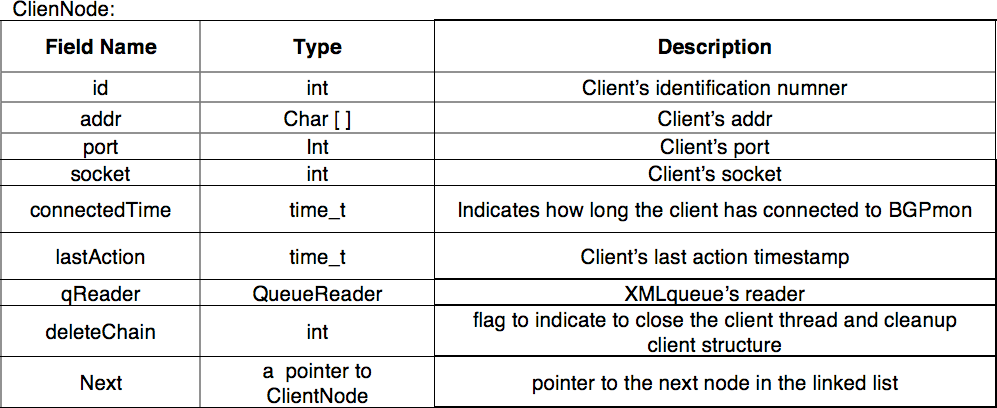
\includegraphics{figs/ClientsctrlNode.pdf}}
\caption{ Client Structure }
\label{fig:clientsctrl:struct:node}
\end{figure*}
\end{itemize}
Note the client thread might exit by itself because of the following 2 reasons:
\begin{itemize}
	\item{ This client thread fails to read the messages from XML queue. In this case, the client thread needs to exit. }
	\item{  This client thread fails to write messages to "socket".}
\end{itemize}
The client thread also might be deleted(call deleteClient) by command line interface(CLI) at running time. Note deleting a client thread is asynchronous action. In other words,  "deleteClient" function only sets the "deleteClient" flag as TRUE. This deletion will be deferred to the next time the child thread checks the "deleteClient" flag. At that time the client thread will exit and the client info in the linked list will be removed. 


\subsection{Design Philosophy}
The important design decision here is that we should let each client specify what they want to receive from BGPmon or we just make BGPmon blindly send everything to the every client.
In the previous design, we did let clients submit their own filters to specify what kind of data they want to receive from BGPmon. But then we realized it would be a huge burden if hundreds of clients all specify their own complex filters.
As our main deign principle is to let BGPmon provide a real-time event stream to a large number of clients, we should relieve BGPmon from the huge burden of handling clients' filters.  As a result, in current design BGPmon simply sends all data to all clients without any processing.  

\section{BGPmon Chains}
\label{sec:chains}


\section{Queue Module}
\label{sec:queue}
Queue is a utility module which is used by other modules to send messages from one to another. As shown in Figure \ref{fig:architecture}, there are 3 queues in BGPMon.
\begin{itemize}
	\item{\emph{ Peer Queue:} It is used by peering module to send internal messages with type 1,2,4 and 6 to the rib and labeling module.}
	\item{\emph{ Label Queue:} It is used by rib and labeling module, periodic module and main module to send all eight types of internal messages to XML generation module. }
	\item{\emph{ XML Queue:} It is used by XML generation module to send XML messages to client management module which in turn sends them to client applications.}
\end{itemize} 
Each of them is a running instance of queue module. They are created by main module during the initial phase of BGPmon and then used by other modules.

The queue module is build on a circular array and each item in this array contains a generic pointer which points to the real message. In this way we can make queue module generic enough to hold all kinds of messages. It also keeps track all the readers and writers. The main data structure of queue module will be introduced in subsection \ref{sub:queue:struct}.

The queue module implements a Readers/Writers pattern where multiple threads may access the same queue simultaneously, some reading and some writing. We call the reading thread reader and the writing thread writer. Each message written by a writer is available to all the readers and a message can be deleted from the queue only after all the readers read it. A key design issue is the locking mechanism to synchronize access to the share data structure in the queue among all threads.  The details of thread synchronization will be discussed in subsection 
\ref{sub:queue:sync}.
 
The biggest challenge in the design of queue module is to avoid being overwhelmed with limited queue length.  There are two situations we need to address: 1) writers write too fast, and 2) Readers read too slow. We will discuss how to address these two situations in subsection \ref{sub:queue:control}.
 
 
\subsection{\label{sub:queue:struct}{Main Data Structure}}
The main data structure of queue module is called 'Queue'. It consists of four parts:
\begin{itemize}
	 \item{\emph{ General Substructure:} It holds the general information for this queue such as the queue's name, its mutex lock and some logging information. See the details in \ref{sub:queue:struct:general}.}
	\item{\emph{ Items Substructure:} It contains all the data of the queue. It implements a circular array. See the details in \ref{sub:queue:struct:items}.}
	\item{\emph{ Readers Substructure:} It contains the information of all readers of the queue. For example, the sequence number of the next unread item for each reader needs to be maintained here. See the details in \ref{sub:queue:struct:readers}.}
	 \item{\emph{ Writer and Pacing Substructure:} It is used to track all the writers in order to pace them when needed. And some other information needed for pacing are also included here such as pacing on/off threshold.  See the details in \ref{sub:queue:struct:writers}.}
\end{itemize}  

\subsubsection{\label{sub:queue:struct:general}{General Substructure}}
The general substructure has the following fields:
\begin{itemize}
	\item{\emph{name:} It is the name of the queue. In BGPmon, the name of peer queue is 'PeerQueue', the name of lable queue is 'LabelQueue' and the name of XML queue is 'XMLQueue'. }
	\item{\emph{ queueLock:} It is a pthread mutex lock which is used for thread synchronization.}
	\item{\emph{ queuecond:} It is a pthread condition variable which is used to notify a reader when the new item gets wrote.}
	\item{\emph{ logging related fields:} A group of logging related fields such as the historical max number of messages, the historical max number of readers and the historical max number of writers.}
	\end{itemize}
Figure \ref{fig:queue:struct:general} shows the details.
\begin{figure*}
\centering
\scalebox{1}{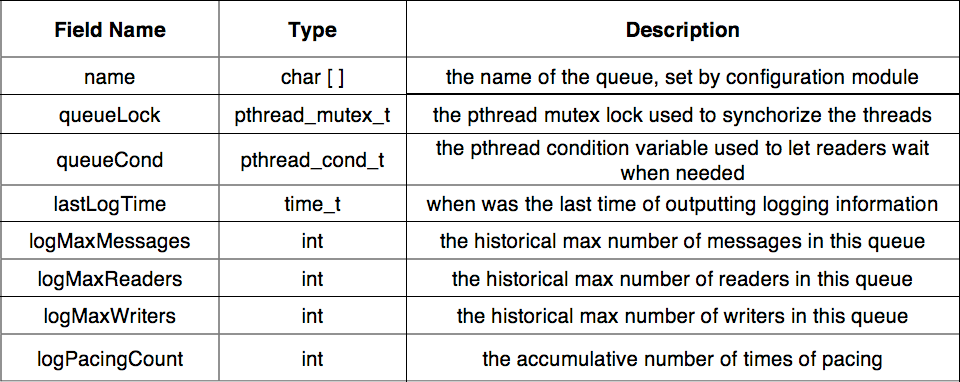
\includegraphics{figs/QueueStructGeneral.pdf}}
\caption{ General Substructure of Queue}
\label{fig:queue:struct:general}
\end{figure*}
	 

\subsubsection{\label{sub:queue:struct:items}{Items Substructure}}
Items substructure maintains a circular array of items which is the heart of queue module. 
Each item is defined as a 'QueueEntry' structure which has the following two fields:
\begin{itemize}
	\item{\emph{count:} It indicates how many readers haven't read it.   This reference count decrements by one after one reader reads this item. If the reference count of a item is zero, this item can be reclaimed by the queue module. Otherwise this item cannot be reclaimed.}
	\item{\emph{messageBuf(void *):} It points to the real data buffer of this item. The data buffer must be created by writers and be passed into queue module.}
\end{itemize}
Items substructure has the following five fields:
\begin{itemize}
	  \item{\emph{head:} It is the sequence number of the oldest item in the queue. It means at least one reader hasn't read this item. The 'head' is incremented after the oldest data item is read by the last reader. }
	  \item{\emph{tail:} It is the sequence number of the next available item in the queue. It is incremented by writing a new message into the queue. }
	  \item{\emph{items:} It is an array of items. Each item is a 'QueueEntry' structure.}
	  \item{\emph{ copy:} It is a callback function. If a reader reads a item and it is not the last reader for this item, the callback function will be called to return a copy of this item to the reader. If a reader is the last one of a item, this item will be returned directly. This allows the reader to always free the returned item after processing it without knowing the details of queue. }
	  \item{\emph{ sizeof:} It is a callback function. Based on 'QueueEntry' structure, we know the size of a item depends the size of its data buffer. This function is used to get the size of a data buffer in bytes. As the data format is queue specific, the sizeof function is provided by the queue creator.}
\end{itemize}
In order to avoid drop any messages in the queue, the different between 'head' and 'tail' must be smaller than 'max' field. Note 'head' and 'tail' are all sequence numbers, not subscripts of array. A sequence number(seq) is long integer and is a logical subscript of the queue. The subscript to access the physical array can be calculated by seq \% max.
Figure \ref{fig:queue:struct:items} shows the details of this substructure.
\begin{figure*}
\centering
\scalebox{1}{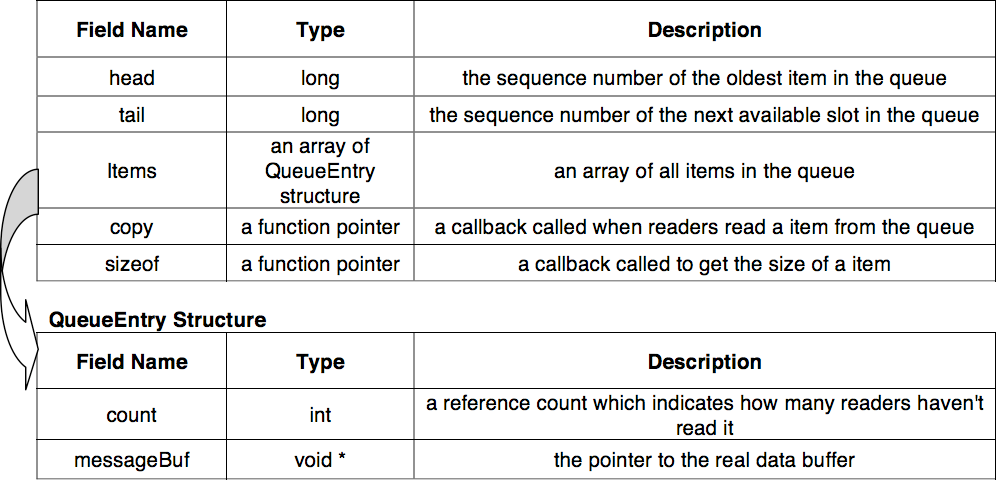
\includegraphics{figs/QueueStructItems.pdf}}
\caption{ Items Substructure of Queue}
\label{fig:queue:struct:items}
\end{figure*}
	 

\subsubsection{\label{sub:queue:struct:readers}{Readers Substructure}}
This substructure is used to track all the readers. It has the following three fields:
\begin{itemize}
	\item{\emph{readerCount:} It is the current number of readers. }
	\item{\emph{nextItem:} It is an array of sequence numbers for all the readers. This array is indexed by reader ID and each sequence number indicates the next unread item in the queue for the corresponding reader. For example, nextItem[6] is the sequence number of the next unread item for the reader with ID 6. The length of this array equals the max number of readers. }
		\item{\emph{itemsRead:}  This array is indexed by reader ID and each element indicates total items read by the corresponding reader. For example, itemsRead[6] is the number of total read items by the reader with ID 6. The length of this array also equals the max number of readers. }
\end{itemize}	
Note the readers of the same queue might have different next item. 


Figure \ref{fig:queue:example} shows an example of the queue which can help us understand the items substructure and readers substructrure.
\begin{figure}[!htb]
\centering
\scalebox{0.44}{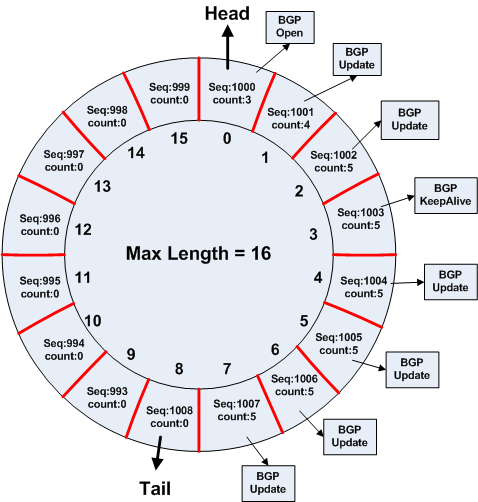
\includegraphics{figs/QueueExample.png}}
\caption{ An Example of Queue}
\label{fig:queue:example}
\end{figure}
In this example, there are a queue with max length 16 and 5 readers. The items substructure looks like this:
\begin{itemize}
	\item{\emph{head:} is 1000 which is sequence number of the oldest item. The count of that item is 3 which means there are three readers haven't read it. }
	  \item{\emph{tail:} is 1008 which is sequence number of the next available item for the new message. }
	  \item{\emph{items:} It is an array of 16 items. 8 of them are in use. }
	  \begin{itemize}
	  	\item{The item with sequence number 1000 has a reference count as 3 which means 3 readers haven't read it.}
		 \item{The item with sequence number 1001 has a reference count as 4 which means 4 readers haven't read it.}
		 \item{All the others item with sequence number from 1002 to 1007 has a reference count as 5 which means all 5 readers haven't read it.}
	\end{itemize}
\end{itemize} 

The corresponding readers substructure is as follows:
\begin{itemize}
	\item{\emph{readerCount:} is 5 which means there are 5 readers.}
	  \item{\emph{nexItem[0]:} is 1000 which means the next item for the reader 0 is 1000 .}
	   \item{\emph{nexItem[1]:} is 1000 which means the next item for the reader 1 is 1000 .}
	    \item{\emph{nexItem[2]:} is 1000 which means the next item for the reader 2 is 1000 .}
	     \item{\emph{nexItem[3]:} is 1001 which means the next item for the reader 3 is 1001 .}
	      \item{\emph{nexItem[4]:} is 1002 which means the next item for the reader 4 is 1002 .}
	      
	     	  \item{\emph{itemsRead[0]:} is 0 which means reader 0 hasn't read anything .}
	   \item{\emph{itemsRead[1]:} is 0 which means reader 1 hasn't read anything.}
	    \item{\emph{itemsRead[2]:} is 0 which means reader 2 hasn't read anything.}
	     \item{\emph{itemsRead[3]:} is 1 which means reader 3 has read 1 items.}
	      \item{\emph{itemsRead[4]:} is 2 which means reader 4 has read 2 items.} 
\end{itemize} 


\subsubsection{\label{sub:queue:struct:writers}{Writers and Pacing Substructure}}
This structure is used to track the writing rate of all the writers and pace them when needed. It has the following fields:
 \begin{itemize}	
 	\item{\emph{writerCount:} It is the number of current writers.}
	  \item{\emph{tick:} It is the start time of the current pacing interval.}
	  	\item{\emph{readCount:} It is used together with 'tick' to count how many messages are read in one interval by all the readers. }
	\item{\emph{writeCounts:} It is an array of counts for all the writers. One count is for each writer which is used together with 'tick' to count how many messages are written in one interval. The length of this array equals the max number of writers.}
	\item{\emph{writesLimit:} It is how many messages are allowed to be written in the queue by each writer in one interval when pacing is turned on. }
	\item{\emph{pacingFlag:} It is set to TRUE if pacing is turned on. It is set to FALSE if pacing is turned off.} 
\end{itemize} 
Figure \ref{fig:queue:struct:writers} shows the details of this substructure.
\begin{figure*}
\centering
\scalebox{1}{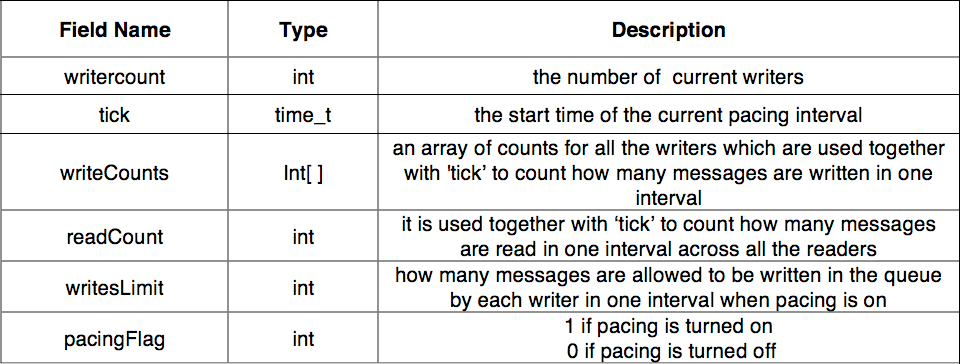
\includegraphics{figs/QueueStructWriters.pdf}}
\caption{ Writers and Pacing Substructure of Queue}
\label{fig:queue:struct:writers}
\end{figure*}
In the subsection \ref{sub:queue:control}, we will discuss how pacing works by using this substructure in detail.
 
\subsection{\label{sub:queue:sync}{Thread Synchronization}}
In BGPmon, there are multiple writers that write messages into one queue and multiple readers that read messages from the same queue. As each read/writer is a separate thread, the thread synchronization is very important for the queue. In our design we use mutex lock and condition variable to manage the thread synchronization. Basically the writer needs to lock the queue by obtaining 'queuelock' in general substructure before it writes a message and unlock the queue by release  'queuelock'  after it writes a message. Similarly the reader needs to lock the queue before it reads a message and unlock the queue after it reads a message.

When a reader exhausts the messages in the queue, it must wait for new messages while other readers or writers still need to continue their reading or writing. In our design, if a reader wants to read a message from the queue and successfully locks the queue by obtaining 'queuelock', it will do the following checks:
 \begin{itemize}	
 	\item{If there are some new messages available for it to read, it will read the oldest one and unlock the queue.}
	\item{Otherwise, it unlocks the queue and waits on the condition variable 'queueCond' to lock the queue again. If any writer writes any new messages into the queue, the queue will broadcast this condition to all the waiting readers.}
\end{itemize} 

\subsection{Interface Functions}
In the queue module, there are only two interface functions which can be used by other modules.
 \begin{itemize}	
 	\item{\emph{readQueue:} It is used to read a message from queue by giving a queue ID, reader ID and a pointer which points to the result data buffer. The return value of 'readQueue' is the number of remaining messages of this reader. It may return READER\_SLOT\_AVAILABLE if this reader has ceased. See details in \ref{sub:queue:control:adjust}}.
	\item{\emph{writeQueue:}  It is used to write a message into queue by giving a queue ID, writer ID and a pointer which points to the written message. It returns 0 if successes.}
\end{itemize}  

\subsection{\label{sub:queue:control}{Stream Control}}
In our design, the queue removes a message until all the readers read it. As a result there are two things we can do in order to prevent a queue being overwhelmed.
\begin{itemize}
	\item{\emph{Pacing writers:} The queue paces the writers according to the average reading rate across all the readers. For example the queue is almost full and there are 4 readers and 2 writers. If each of reader can read 8 messages per second averagely, we should limit the writing rate of each writer to 8/2 = 4 in order to avoid overwhelm the queue.  See details in \ref{sub:queue:control:pacing}.}
	\item{\emph{Adjust slow readers:} In some cases pacing writers doesn't work, the queue needs to adjust the slow readers. For example, the queue is almost full and there are 4 readers and 2 writers. If 3 of the 4 readers can read 8 messages per second but one of them can only read 2 message per second. As a result, the average reading rate across the 4 readers is 6.5 messages per second. In this case, even pacing is turned on and each writer is limited to write 6.5/2 = 3.25 messages per second the queue will still be overwhelmed because the slowest reader cannot read 3.25 messages per second. That's why in this case the queue has to adjust the slowest reader by skipping its unread items. See details in \ref{sub:queue:control:adjust}.}
\end{itemize} 

\subsubsection{\label{sub:queue:control:pacing}{Pacing Writers}}
In our design, the queue utilization(from 0\% to 100\%) is used to determine when to turn on pacing.  When the queue utilization exceeds a configurable threshold(PacingOnThreshold), pacing is turned on until the queue utilization drops below a configurable threshold(PacingOffThreshold).  The reason why we have two thresholds here is this allows the queue to reach a steady state rather than oscillate in and out of pacing.
During the pacing period, the objective is to make the writers write at a pace that matches the average reader. More specifically, in each configurable interval(PacingInterval) the queue limits the number of writes from each writer according to the average number of reads by all readers. 
In order to do this,  when a new interval starts we need to predict the number of reads by all readers in this new interval and then use this value to pace the writers in this new interval.   
The pacing related logic related to the 'readQueue' function is as follows:
\begin{enumerate}
	\item{Check if a new interval starts}
		\begin{enumerate}
		\item{If yes,  update the 'writesLimit' using exponential weighted moving average(EWMA):}
				\begin{enumerate}
					\item{Calculate the new 'writesLimit' by this formula. Note 'alpha' is configurable, 'writesLimit' is the number if writes allowed per writer in the new interval, 'averageReads' is the average number of reads by all readers in the past interval and 'writerCount' is the number of writers.}						
								\begin{eqnarray*}
writesLimit&=& (1-alpha) * writesLimit + \\ 
alpha *  \frac{averageReads}{writerCount}
						\end{eqnarray*}
						\item{If new 'writesLimit' is larger than half of the remaining queue, use half of the remaining queue as the new 'writesLimit'. }
					\item{If new 'writesLimit' is smaller than a configurable 'minWritesLimit', use 'minWritesLimit' as the new 'writesLimit'. }
				\end{enumerate}
		\item{Otherwise, do nothing.}
		\end{enumerate}
		\item{Check if needs to turn off pacing by compare the queue utilization with the configurable threshold(PacingOffThreshold).}
		\begin{enumerate}
			\item{If the queue utilization is smaller, set the 'pacingFlag' field as FALSE. }
			\item{Otherwise, do nothing.}
		\end{enumerate}
\end{enumerate}
Note this logic will be executed every time a reader calls 'readQueue'.

The 'writeQueue' function starts with the same pacing related logic as 'readQueue'. But after that, it needs to limit the number of writes per interval according to the 'writersLimit' field when pacing is enabled. This additional step inside the 'writeQueue' function is as follows:
\begin{enumerate}	
	\item{Check if needs to turn on pacing by compare the queue utilization with the configurable threshold(PacingOnThreshold).}
			\begin{enumerate}
			\item{If the queue utilization is larger, set the 'pacingFlag' field as TRUE. }
			\item{Otherwise, do nothing.}
			\end{enumerate}
			
	\item{Check if 'pacingFlag' is set to TRUE. }
		\begin{enumerate}
		\item{If yes,  do the following checks:}
				\begin{enumerate}
					\item{If 'writeCount[writerID]' is larger than 'writesLimit', sleep until a new interval starts.}
					\item{Otherwise, do nothing.}
				\end{enumerate}									
		\item{Otherwise, do nothing.}
		\end{enumerate}
\end{enumerate}
This logic will be executed every time a writer calls 'writeQueue'.
  
\subsubsection{\label{sub:queue:control:adjust}{Adjust Slow Readers}}
Pacing prevents the queue from being overwhelmed if the readers are uniformly able to read the messages at the same rate.  In the case of a slow reader, the queue utilization will still continue to grow.  When the queue utilization reaches the maximum, the responsible reader is adjusted by skipping all its unread items.
This logic is mainly implemented in the 'writeQueue' function.
\begin{enumerate}
	  \item{Check if the queue is full.}
	     \begin{enumerate}
	     \item{If it is full, find the slowest reader and adjust it by skipping all its unread items. For each reader, check the nextItem[readerID] as follows:}
	     		\begin{enumerate}
	     			\item{ If nextItem[readerID] equals to 'head', adjust this reader as mentioned.}
			\end{enumerate}	
	     \end{enumerate}
\end{enumerate}

In the 'readQueue' function, suppose the queueID, readerID and a pointer is passed in from a caller.
\begin{enumerate}
	\item{If head <= nextItem[readerID] < tail , pass the oldest message to the caller via the pointer and return the number of remaining messages.}
	\item{If nextItem[readerID] >= tail,block the caller until a new message is written into the queue. }
	\item{If nextItem[readerID] = READER\_SLOT\_AVAILABLE , it means the reader has ceased and return READER\_SLOT\_AVAILABLE to the caller.}
\end{enumerate}
If a caller receives READER\_SLOT\_AVAILABLE from 'readQueue', that means the corresponding reader has ceased. Then the caller may need to close thread and release resources in this case.

\subsection{Design Philosophy}
The most important design issue here is how to handle slow readers.  As we discussed, it is essential that some action be taken to address the problem of slow readers. If no action is taken,  a slow reader can cause the queue to overflow and eventually data would be dropped.   This is particularly problematic if most readers could read at a high rate and receive all the data, but a few slow readers fill the queues and cause data loss.   

In the previous design, our solution is to identify and then terminate the slow readers.  However, by doing that a potential problem is that the slow reader may simply re-connect and thus drive the overall system into a state of persistent oscillation.    The system runs well until the slow reader joins.   The slow reader then causes queues to build up and the reader is eventually killed.   The queue then quickly drains when the slow reader is killed.   Note that the queue contains at least one update that has been read by everyone except the slow reader.    When the slow reader is killed, that update can be discarded.    In our experiments thus far, a typical slow reader has hundreds of updates that are waiting only for the slow reader;  killing the slow reader immediately removes these updates and frees hundreds of slots in the queue.   But oscillation occurs if the slow reader immediately connects.    The queue of unread updates begins to build again as soon as the slow reader joins and the cycle repeats.   One can easily imagine a poorly written slow reader that automatically reconnects anytime it is disconnected.

An alternate approach is to better manage, but not kill the slow readers.   In current design, the slow reader is not deleted from the system.   Instead, slow readers are forced to skip messages.     From a queuing standpoint, the effect is similar to killing the slow reader and works as follows.   When BGPmon determines a reader is reading messages too slowly,  all messages that have yet to be read by that slow reader are immediately marked as read.    In this case the slow reader misses several messages, but it is allowed to continue. 




\section{Login Module}
\label{sec:login}

The login module handles the Cisco-like commands typed by logined users and calls the corresponding functions provided by other modules. It is made up of several pieces.  

The first piece is a listener that listens on a specific address and port for new Command Line Interface (CLI) connections.  Once a connection has been established then the next major piece, the command tree structure, is used.  This structure is a tree ADT that contains a complete mapping of all the commands that can be called from the CLI.  Each command is broken down into parts and each part is added to the tree.  For instance the command 'show running' is broken into two pieces.  The 'show' command is a child of the root node and the 'running' command is child of the 'show' command.  When a command is executed from the CLI, the command is sent from the client to the server then broken down and mapped into the command structure.  If the entire command can be mapped onto the tree then the final node will contain a function pointer for the command.  Every node in the structure also has an associated mask with it that controls whether the command is visible or executable to a given security level.  All the commands have been organized in a way that will help make maintenance of them easier.  In commandprompt.c there are a series of functions that contain the necessary code to create the commands and associations to the necessary functions.  Then, there is a series of files that end with '\_commands.c' which contain the functions for each module that the commands reference.
%\section{Conclusion}
\label{sec:conclude}

Overall, we believe BGPmon represents an important change in how BGP route monitoring is accomplished in the Internet. We hope that the addition of BGPmon will make it much simpler for researchers and operators to obtain BGP data and the addition of widely available real-time BGP data will lead to the development of new tools for better understanding Internet routing. If you would like to know more about the BGPmon project, please visit our web page \emph{http://bgpmon.netsec.colostate.edu} or contact the public maillist \emph{bgpmon@netsec.colostate.edu}

\section{Acknowledgements}
\label{sec:ack}




\bibliographystyle{abbrv}
\bibliography{sigproc}

%\appendix

\end{document}
